\documentclass{article}
\usepackage[a4paper, total={170mm, 257mm}, left=20mm, right=20mm, top=10mm]{geometry}

\usepackage{amsmath, amsthm, amssymb, amsfonts}
\usepackage{thmtools}
\usepackage{graphicx}
\usepackage{caption, subcaption}
\usepackage{setspace}
\usepackage{float}
\usepackage[colorlinks=true, linkcolor=blue]{hyperref}
\usepackage[utf8]{inputenc}
\usepackage[english]{babel}
\usepackage{framed}
\usepackage[dvipsnames]{xcolor}
\usepackage{tcolorbox}
\usepackage{subcaption}
\usepackage{amssymb}
\usepackage{cite}
\usepackage{booktabs}
\usepackage{multirow}
\usepackage{anyfontsize}
\usepackage{tabularx}
\usepackage{adjustbox}
\usepackage{abstract}
\usepackage{array}

\colorlet{LightGray}{White!90!Periwinkle}
\colorlet{LightOrange}{Orange!15}
\colorlet{LightGreen}{Green!15}

\newcommand{\HRule}[1]{\rule{\linewidth}{#1}}

\declaretheoremstyle[name=Theorem,]{thmsty}
\declaretheorem[style=thmsty,numberwithin=section]{theorem}
\tcolorboxenvironment{theorem}{colback=LightGray}

\declaretheoremstyle[name=Proposition,]{prosty}
\declaretheorem[style=prosty,numberlike=theorem]{proposition}
\tcolorboxenvironment{proposition}{colback=LightOrange}

\declaretheoremstyle[name=Principle,]{prcpsty}
\declaretheorem[style=prcpsty,numberlike=theorem]{principle}
\tcolorboxenvironment{principle}{colback=LightGreen}

\setstretch{1.2}
\geometry{
    textheight=9in,
    textwidth=5.5in,
    top=1in,
    headheight=12pt,
    headsep=25pt,
    footskip=30pt
}

% ------------------------------------------------------------------------------

\begin{document}

    % Cover Page and ToC
    \title{ \normalsize \textsc{}
\\ [2.0cm]
\HRule{1.5pt} \\
\LARGE \textbf{\uppercase{Machine Learning and Pattern Recognition Report}
\HRule{2.0pt} \\ [0.6cm] \LARGE{Fingerprint Spoofing Detection} \vspace*{10\baselineskip}}
}
\date{}
\author{\textbf{Antonio Iorio} \\
Who? \\
Where? \\
When?}

\maketitle
\newpage

\tableofcontents
\newpage

    %Introduction

    \paragraph{Introduction}
    The project task consists of a binary classification problem.
    The goal is to perform fingerprint spoofing detection, i.e.\ to identify genuine vs counterfeit fingerprint images.
    The dataset consists of labeled samples corresponding to the genuine (True, label 1) class and the fake (False, label 0) class.
    The samples are computed by a feature extractor that summarizes high-level characteristics of a fingerprint
    image.
    The data is 6-dimensional.

%    Dataset Analysis


    \section{Dataset Analysis}
    \label{sec:datasetAnalysis}
    %! Author = antonio
%! Date = 7/1/24

In our analysis process, one first begins to represent what are the data related to the various features
and how among the various features the data are distributed by making a visual representation in pairs of features.

\begin{enumerate}
%    FEATURE 1 AND 2
    \item Starting with the analysis of the first two features and creating a histogram and a scatter
    \autoref{fig:feature1vs2}, one can see:
    \begin{itemize}
        \item Both features overlap
        \item Follow a Gaussian distribution
        \item Feature 1 has a peak at [-0.213, 0.276] and it is worth 0.541 for the false class, instead for Feature 2
        the peak at [-0.402, 0.165] and it is worth 0.516 for the true class.
    \end{itemize}
    Seeing \autoref{fig:feature1vs2} again, it would appear that \autoref{fig:feature1vs2a} and
    \autoref{fig:feature1vs2b} appear to be visually the same but in b they are represented centred
    which as can be seen is quite similar because Feature 1 has \(\mu = 0.00170711\)
    and \(\sigma^2 = 1.00134304\), instead Feature 2 has \(\mu = 0.00503903\) and \(\sigma^2 =  0.9983527\)
    \begin{figure}[h!]
        \centering
        \begin{subfigure}[b]{0.4\linewidth}
            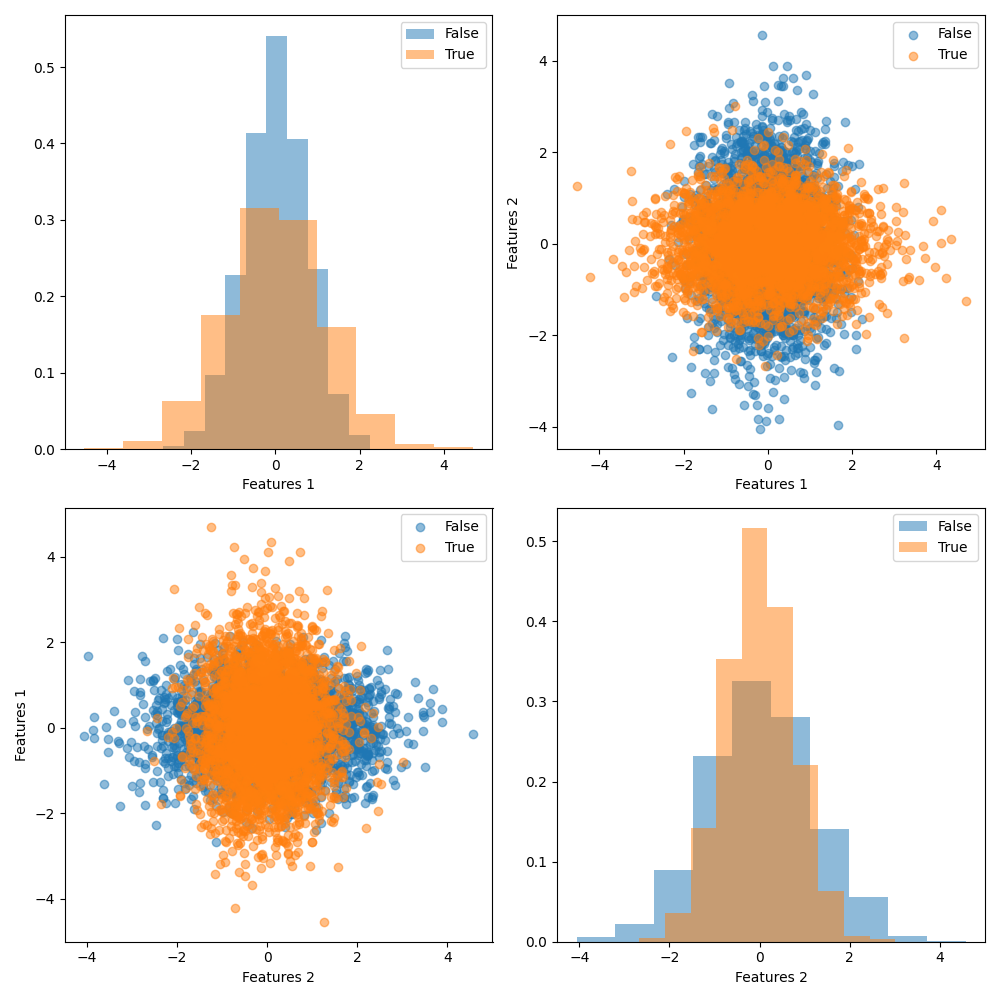
\includegraphics[width=\linewidth]{Lab/02. Lab 02/Images/01. Graphics Features 1_2 Without Mean}
            \caption{Without mean}
            \label{fig:feature1vs2a}
        \end{subfigure}
        \begin{subfigure}[b]{0.4\linewidth}
            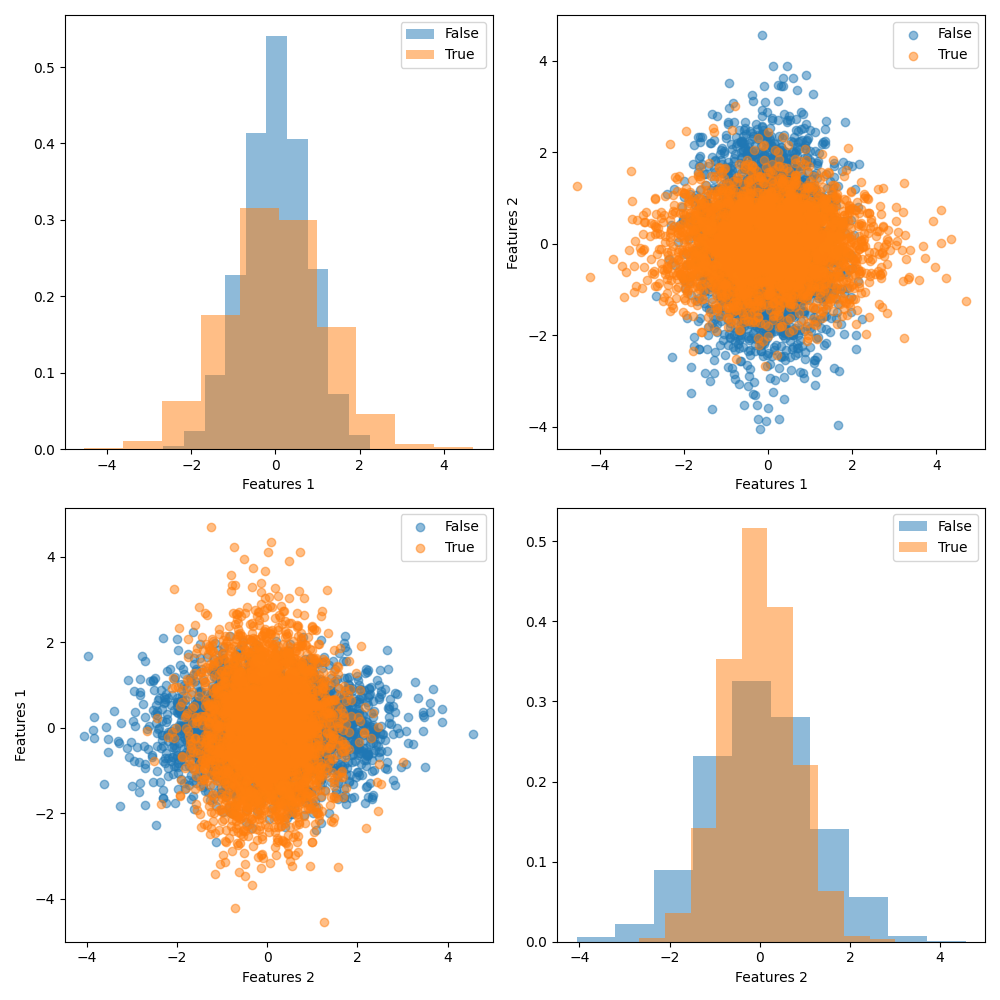
\includegraphics[width=\linewidth]{Lab/02. Lab 02/Images/02. Graphics Features 1_2 With Mean}
            \caption{With mean}
            \label{fig:feature1vs2b}
        \end{subfigure}
        \caption{Feature 1 vs Feature 2 - Without centering the data relative to the average (a)
            and with centering the data relative to the average (b)}
        \label{fig:feature1vs2}
    \end{figure}


%    FEATURE 3 AND 4
    \item For features 3 and 4, observed in \autoref{fig:feature3vs4}, on the other hand, they have:
    \begin{itemize}
        \item do not overlap like the previous two
        \item Follow a Gaussian distribution but the true and false labels are centred at different
        points
        \item Feature 3 has a peak at [-1.063, -0.568] and it is worth 0.517 for the false class,
        instead for Feature 4 the peak at [0.290, 0.783] and it is worth 0.525 for the false class.
    \end{itemize}
    Seeing \autoref{fig:feature3vs4a} and \autoref{fig:feature3vs4b}, data are already similar because, the mean
    calculated with reference to the two classes is close to 0, in fact:
    Feature 3 has \(\mu = -0.00560753\) and \(\sigma^2 = 1.0024818\), instead
    Feature 4 has \(\mu = 0.00109537\) and \(\sigma^2 = 0.99029389\)
    \begin{figure}[h!]
        \centering
        \begin{subfigure}[b]{0.4\linewidth}
            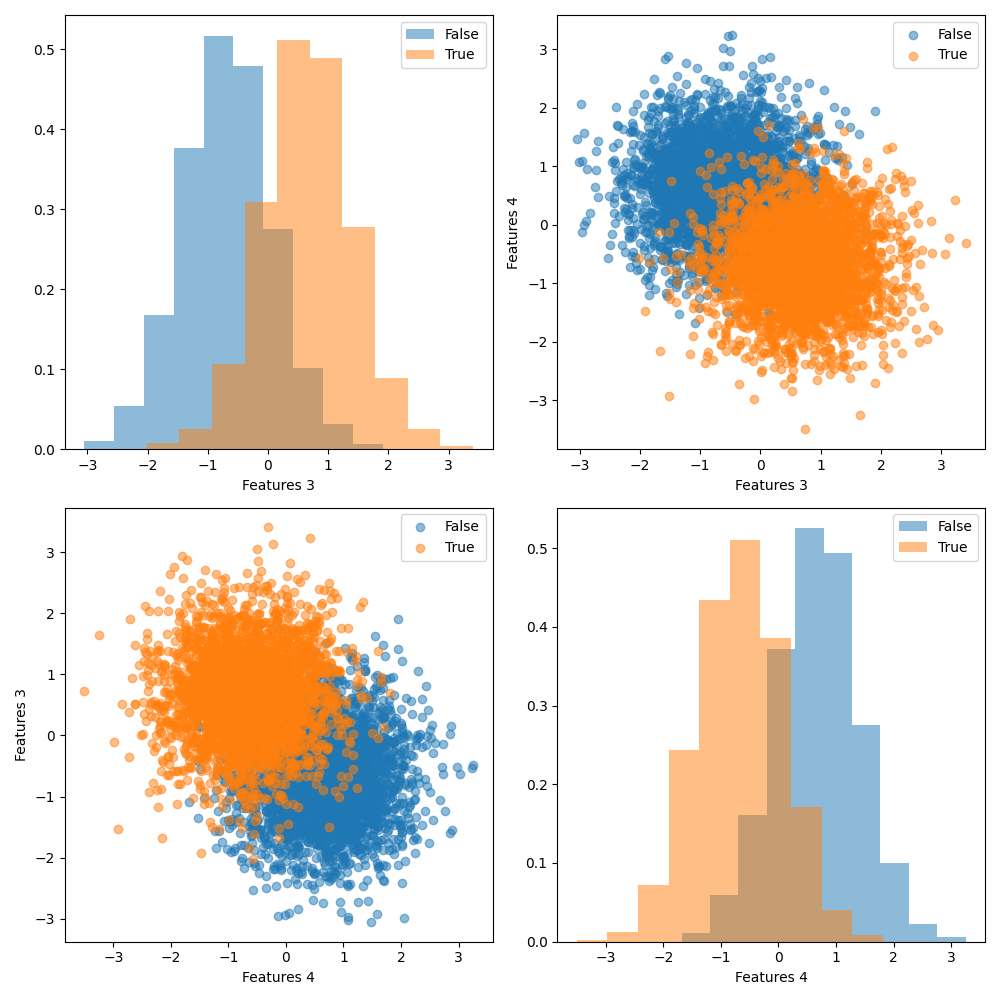
\includegraphics[width=\linewidth]{Lab/02. Lab 02/Images/03. Graphics Features 3_4 Without Mean}
            \caption{Without mean}
            \label{fig:feature3vs4a}
        \end{subfigure}
        \begin{subfigure}[b]{0.4\linewidth}
            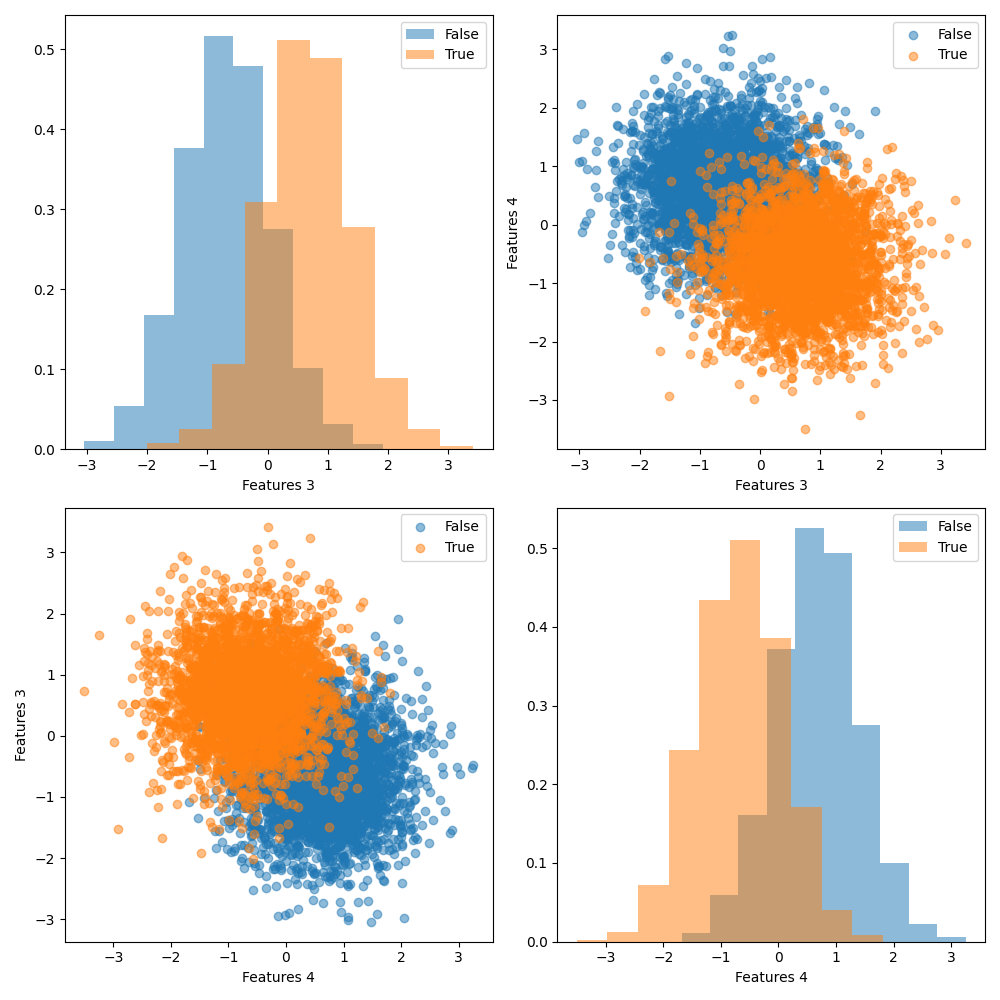
\includegraphics[width=\linewidth]{Lab/02. Lab 02/Images/04. Graphics Features 3_4 With Mean}
            \caption{With mean}
            \label{fig:feature3vs4b}
        \end{subfigure}
        \caption{Feature 3 vs Feature 4 - Without centering the data relative to the average (a)
            and with centering the data relative to the average (b)}
        \label{fig:feature3vs4}
    \end{figure}


%    FEATURE 5 AND 6
    \item  For features 5 and 6, observed in \autoref{fig:feature5vs6}, one can see:
    \begin{itemize}
        \item Do not totally overlap
        \item For both features, the true labels don't follow a Gaussian distribution as opposed to the false ones,
        which could be more approximate
        \item Feature 5 has a peak at [-1.211, -0.783] and it is worth 0.572 for the true class, instead
        for Feature 6 has a peak at [-1.273, -0.817] and it is worth 0.553 for the true class.
    \end{itemize}
    Also in this other case, \autoref{fig:feature5vs6a} and \autoref{fig:feature5vs6b} are similar because again the
    average is close to 0.
    Feature 5 has \(\mu = -0.00700025\) and Feature 6 has \(\mu = 0.00910515\)

    \begin{figure}[t]
        \centering
        \begin{subfigure}[b]{0.4\linewidth}
            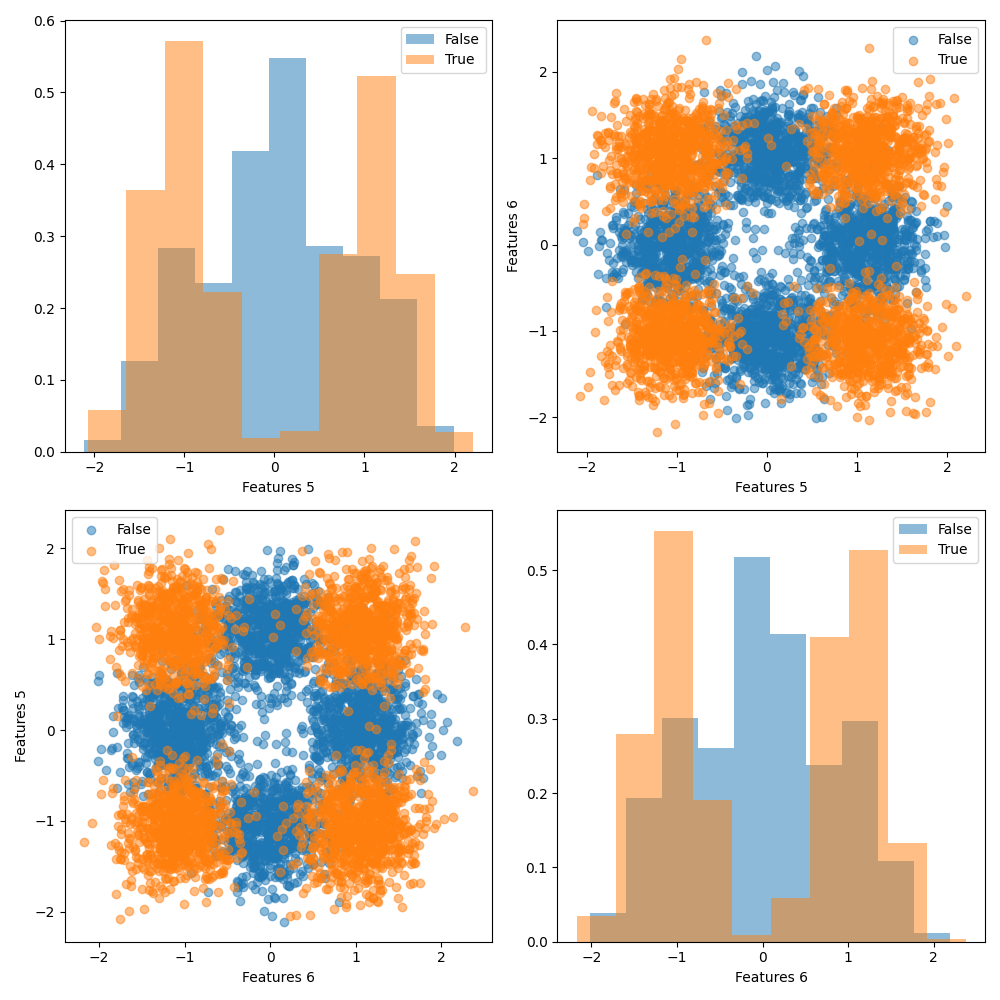
\includegraphics[width=\linewidth]{Lab/02. Lab 02/Images/05. Graphics Features 5_6 Without Mean}
            \caption{Without mean}
            \label{fig:feature5vs6a}
        \end{subfigure}
        \begin{subfigure}[b]{0.4\linewidth}
            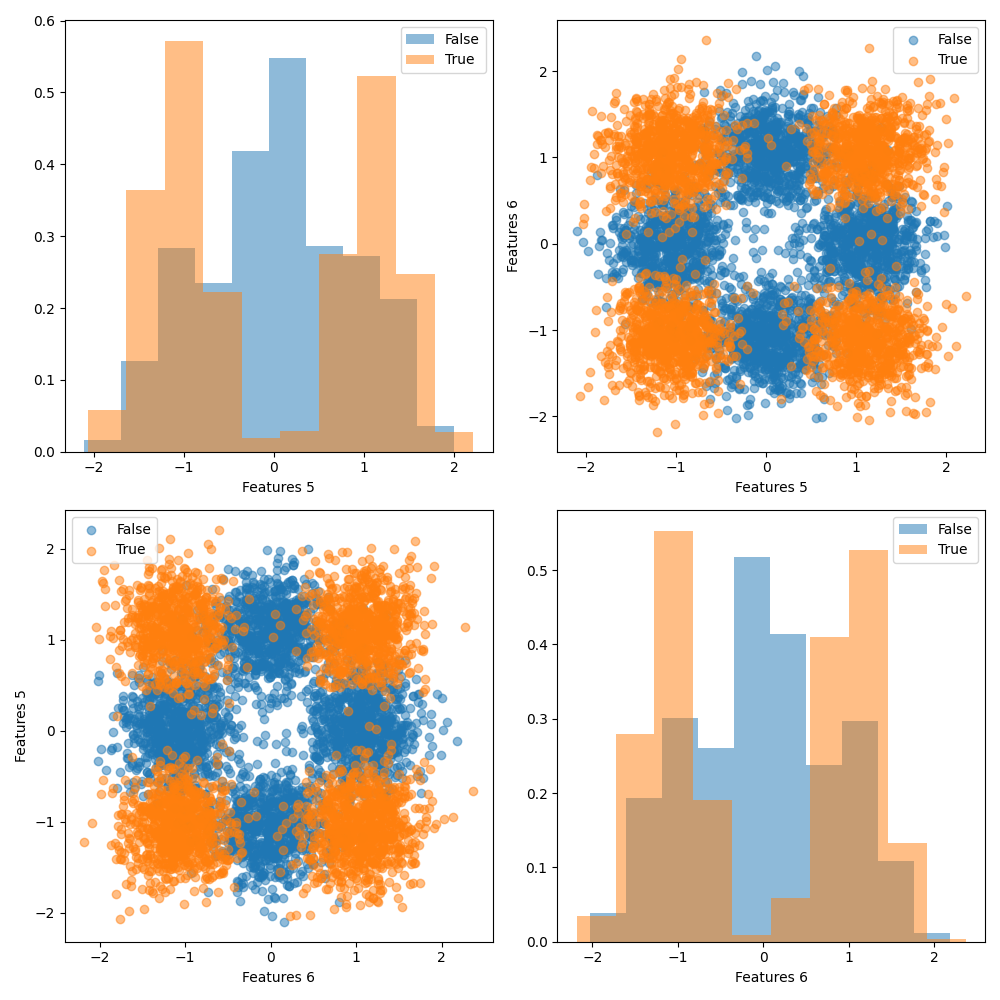
\includegraphics[width=\linewidth]{Lab/02. Lab 02/Images/06. Graphics Features 5_6 With Mean}
            \caption{With mean}
            \label{fig:feature5vs6b}
        \end{subfigure}
        \caption{Feature 5 vs Feature 6 - Without centering the data relative to the average (a)
            and with centering the data relative to the average (b)}
        \label{fig:feature5vs6}
    \end{figure}

\end{enumerate}


%    Dimensionality Reduction


    \section{Dimensionality Reduction}
    \label{sec:dimensionalityReduction}
    %! Author = antonio
%! Date = 7/2/24

Before proceeding with classification, two techniques of dimensionality reduction PCA and LDA can be analysed.
The goal is to find a subspace of the feature space that preserves most of the useful information, that is, mapping from
the \(n\text{–}dimensional\) feature space to \(m\text{–}dimensional\) space, with
\(m \ll n\)

% PCA

\subsection{PCA}
\label{subsec:pca} is an unsupervised technique.
Where starting from a dataset \(X = \{x_1, \dots,x_k\}\) and calculated average.
It starts with the empirical covariance matrix:
\begin{equation}
    C = \frac{1}{K} \sum (x_i - \bar{x})(x_i - \bar{x})^T
    \label{eq:covarianceMatrix}
\end{equation}

We compute the eigen-decomposition of \(C = U \Sigma U^T\) and project the data in the subspace
spanned by the \(m\) columns of \(U\) corresponding to the \(m\) largest eigenvalues.
\begin{equation}
    y_i = P^T(x_i - \bar{x})
    \label{eq:projection}
\end{equation}

where P is the matrix of the \(m\) columns of U associated to the m highest eigenvalues of \(C\).
A cross-validation approach can be used to figure out the optimal value of m to be selected.
To evaluate each eigenvalue, one would have to calculate the variance corresponding to the axis.
The percentage can be calculated as the rate between the sum of the m eigenvalues and the sum of all of them.
In \autoref{fig:percentageVariance} we can see how it changes in the project.
A good m, corresponds to that value which allows a percentage greater than 95\%, so in our case we would need all 6
features.

\begin{figure}[h!]
    \centering
    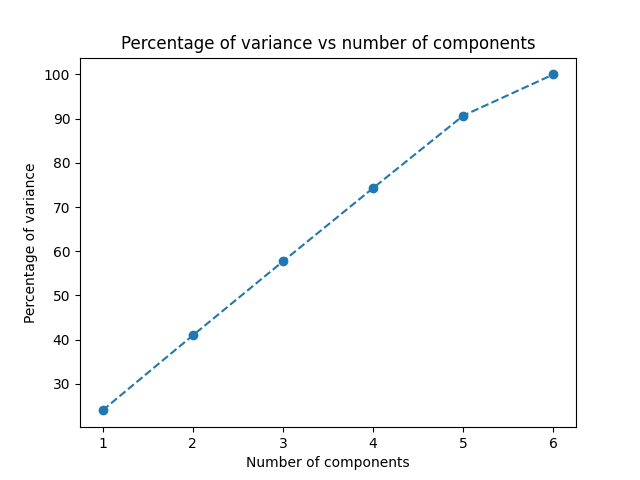
\includegraphics[width=0.5\linewidth]{Lab/03. Lab 03/Images/01. PercentageVariance_NumberOfComponents}
    \caption{Cross validation for PCA impact evaluation}
    \label{fig:percentageVariance}
\end{figure}

% LDA

\subsection{LDA}
\label{subsec:LDA} is a supervised technique.
To find a direction that has the best separation between classes, we measure spread between classes in terms of class covariance.
The objective is to maximize the \(between-class\) variability over \(within-class\) variability ratio for the transformed samples:
\begin{equation}
    \underset{w}{\max} \frac{w^T S_B w}{w^T S_W w}
    \label{eq:ldaFunct}
\end{equation}

where:
\begin{equation}
    S_B  \triangleq \frac{1}{N}\sum_{c=1}^{K} n_c (\mu_c - \mu)(\mu_c - \mu)^T
    \label{eq:betweenClass}
\end{equation}

\begin{equation}
    S_W \triangleq \frac{1}{N}\sum_{c=1}^{K} \sum_{i=1}^{n_c} (x_{c,i} - \mu_c)(x_{c,i} - \mu_c)^T
    \label{eq:withinClass}
\end{equation}

\(\mu\) is dataset mean, \(\mu_{c}\) is class mean, \(n_c\) is the number of samples in class \(c\), and \(N\) is the total number of samples.\\
The directions of LDA can be calculated by solving the generalised eigenvalue problem, as one wants to find the associated eigenvectors \(S_w^{-1}S_b\).
This method allows us to find at most C-1 discriminant directions, where C is the number of classes, since the objective of
LDA is to maximize the separation between classes.
In our case there are 2 classes so there is only one direction

% OUR PROJECT

\subsection{Our project}
\label{subsec:ourProject}
PCA and LDA are applied to the dataset, in particular, m = 6 is used, and in \autoref{fig:pcaLda} we can observe
what are the outcomes for the indicated directions.

\begin{figure}[h]
    \centering
    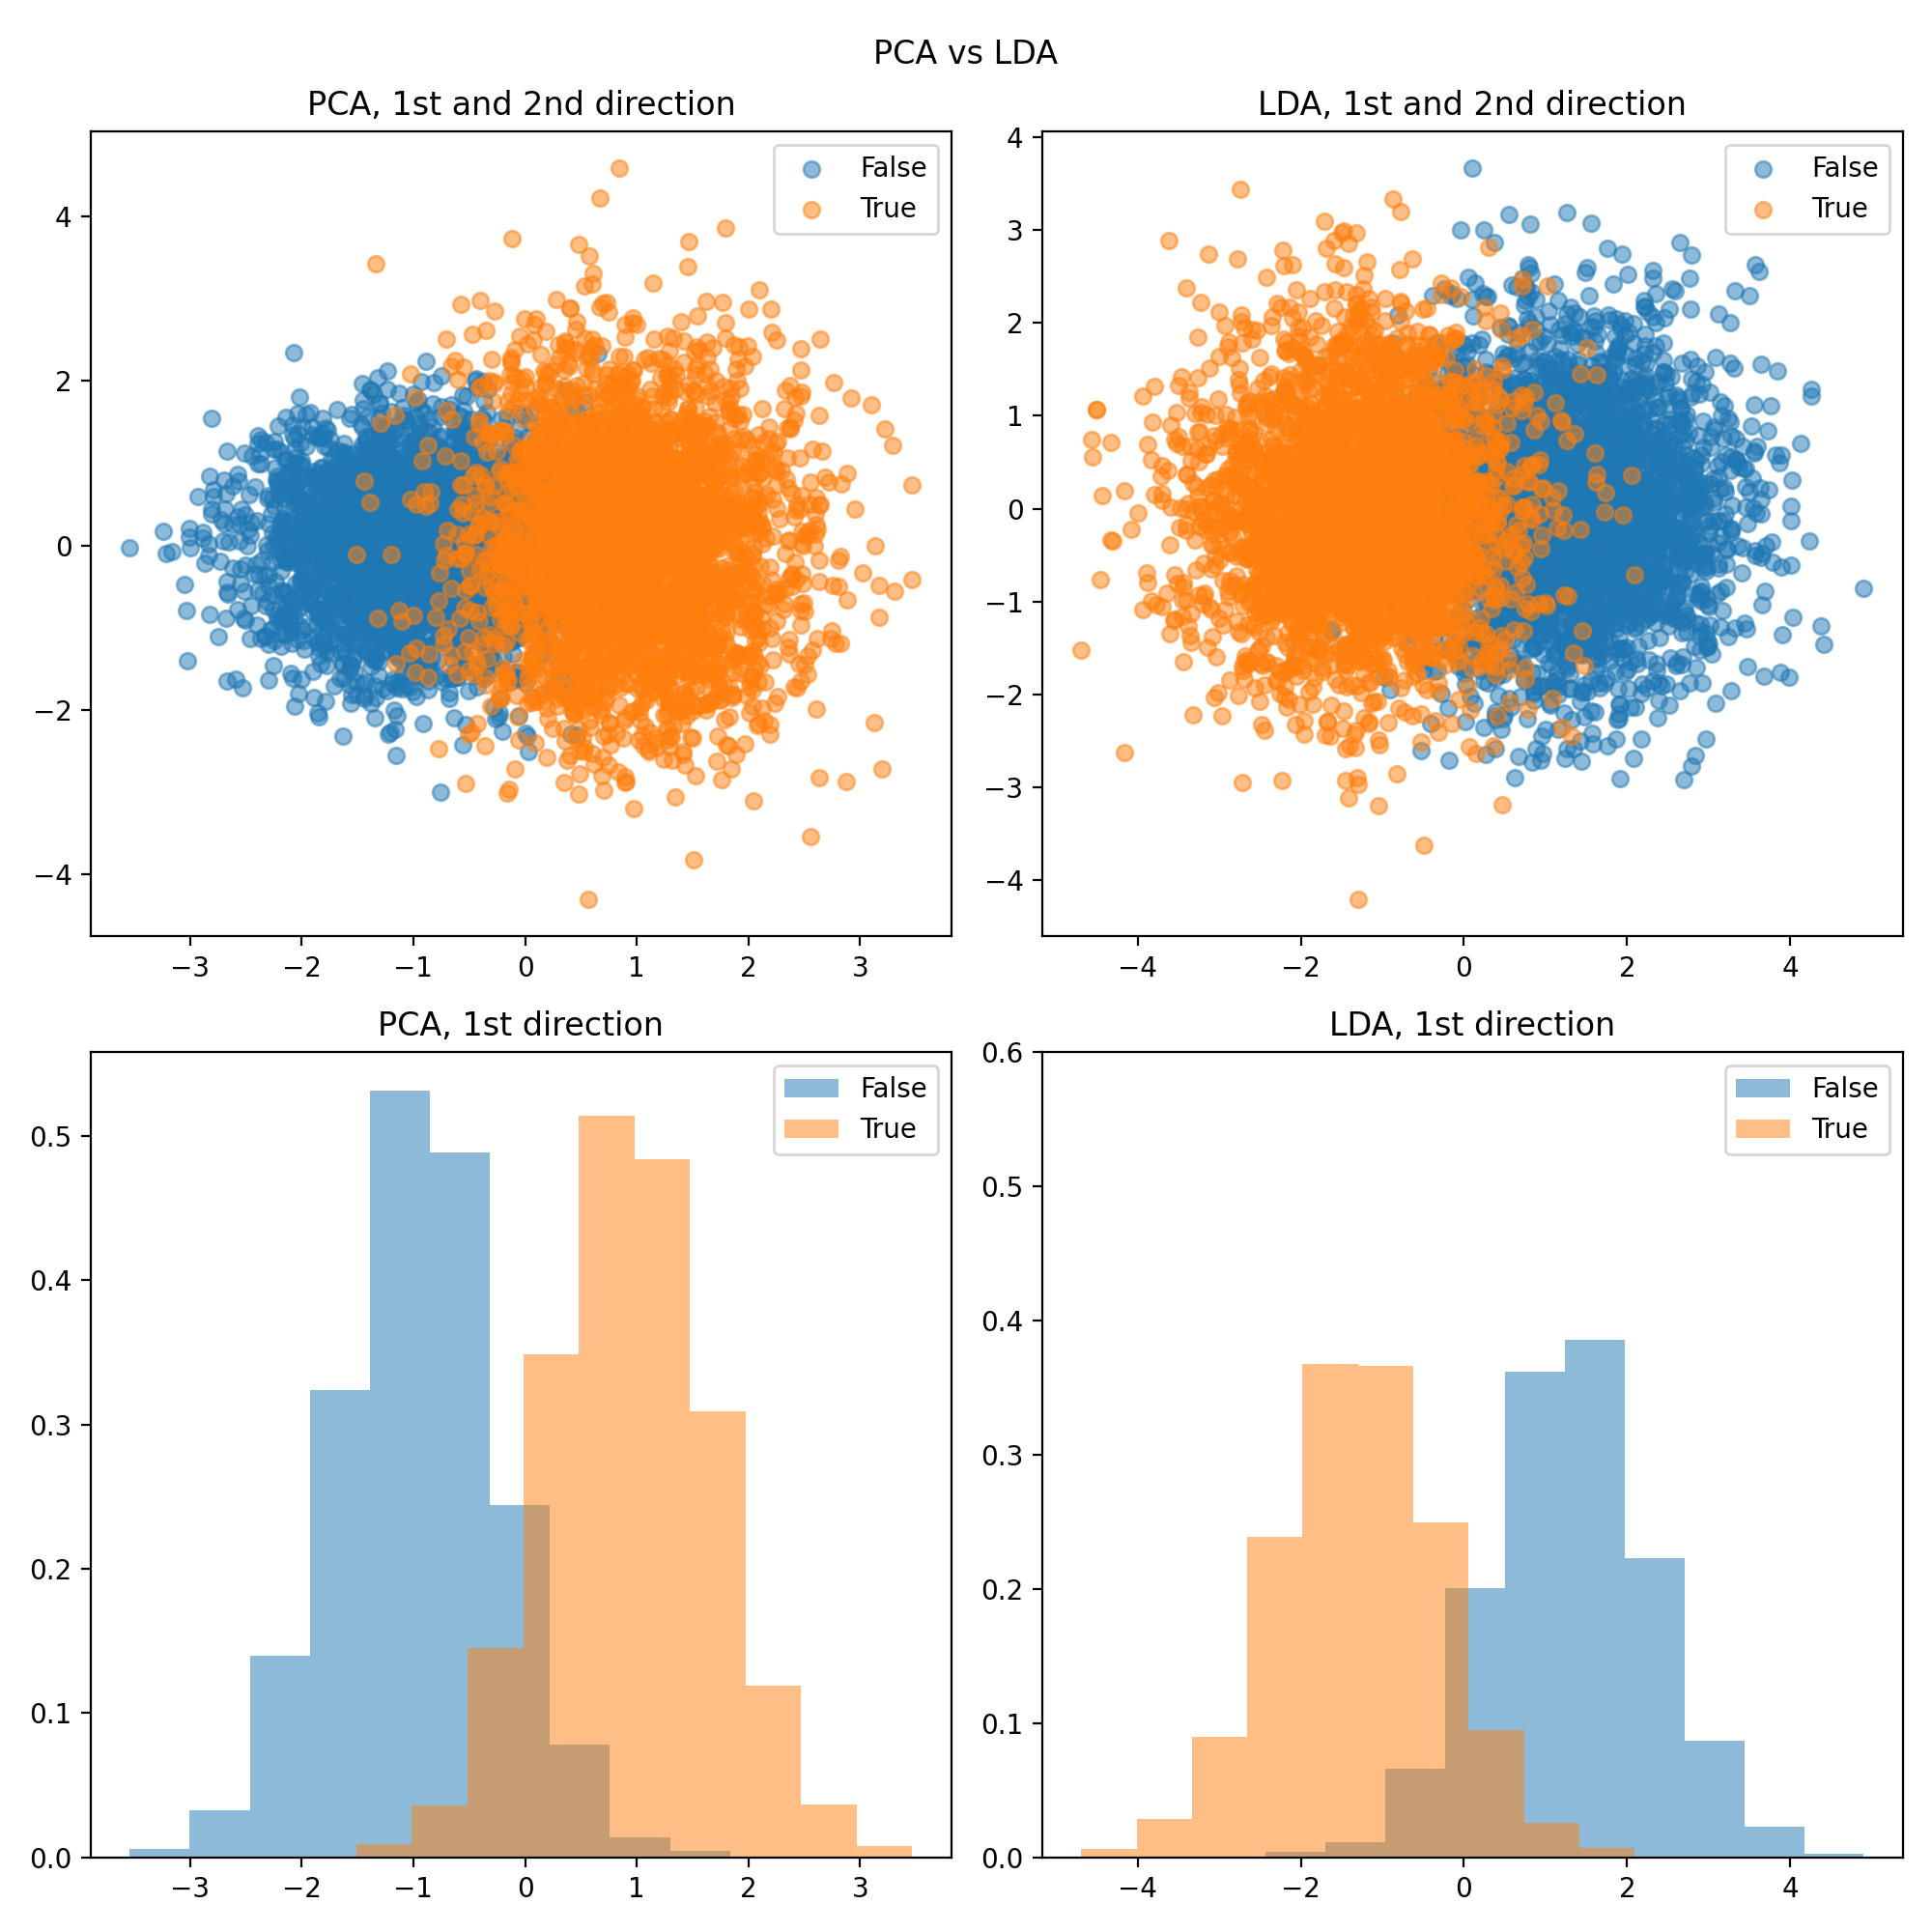
\includegraphics[width=0.5\linewidth]{Lab/03. Lab 03/Images/02. PVA_LDA}
    \caption{Comparing resulta between PCA and LDA}
    \label{fig:pcaLda}
\end{figure}

At a later stage, they were used to carry out a classification.
The available dataset was divided into two sub-portions one for training and the other for validation.
In \autoref{tab:LDAPCAForClassification} we can see the error of the classification,
errors made in the classification when varying m (only for some values) and the threshold were reported

\begin{table}
    \centering
    \begin{tabular}{c c c c}
        \toprule
        \textbf{Method}                    & \textbf{Num Samples} & \textbf{Error} & \textbf{Error Rate} (\%) \\
        \midrule
        LDA - First threshold              & 2000                 & 186            & 9.30                     \\
        LDA - Second threshold             & 2000                 & 186            & 9.30                     \\
        \midrule
        PCA (m=5) + LDA - First threshold  & 2000                 & 186            & 9.30                     \\
        PCA (m=5) + LDA - Second threshold & 2000                 & 185            & 9.25                     \\
        PCA (m=6) + LDA - First threshold  & 2000                 & 186            & 9.30                     \\
        PCA (m=6) + LDA - Second threshold & 2000                 & 184            & 9.20                     \\
        \bottomrule
    \end{tabular}
    \captionsetup{justification=justified,singlelinecheck=false,format=hang}
    \caption{Table showing the results of the LDA and PCA + LDA method for classification.}
    \label{tab:LDAPCAForClassification}
\end{table}










%    Multivariate Gaussian Density


    \section{Multivariate Gaussian Density}
    \label{sec:multivariateGaussianDensity}
    %! Author = antonio
%! Date = 7/2/24

Multivariate Gaussian Density is an extension of the Gaussian Density to multiple dimensions.
It is used to describe the distribution of a vector of random variables in a \(multi-dimensional\) space,
and it could be defined as:
\begin{equation}
    N(x\mid\mu, \Sigma) = \frac{1}{(2\pi)^{\frac{M}{2}} \left|\Sigma \right|^{\frac{1}{2}}}\exp^{-\frac{1}{2}(x-\mu)^T\Sigma^{-1}(x-\mu)}
    \label{eq:gaussianDensity}
\end{equation}

where \(M\) is the size of the feature vector \(x\), and \(\left|\Sigma \right|\) is the determinant of \(\Sigma\).
Since the computation of the exponential could cause problems, the logarithm is applied, so from \autoref{eq:gaussianDensity}
we get \autoref{eq:logGaussianDensity}:

\begin{equation}
    \log N(x\mid\mu, \Sigma) = -\frac{M}{2}\log(2\pi) - \frac{1}{2}\log\left|\Sigma \right| - \frac{1}{2}(x-\mu)^T\Sigma^{-1}(x-\mu)
    \label{eq:logGaussianDensity}
\end{equation}

\begin{figure}[h]
    \centering
    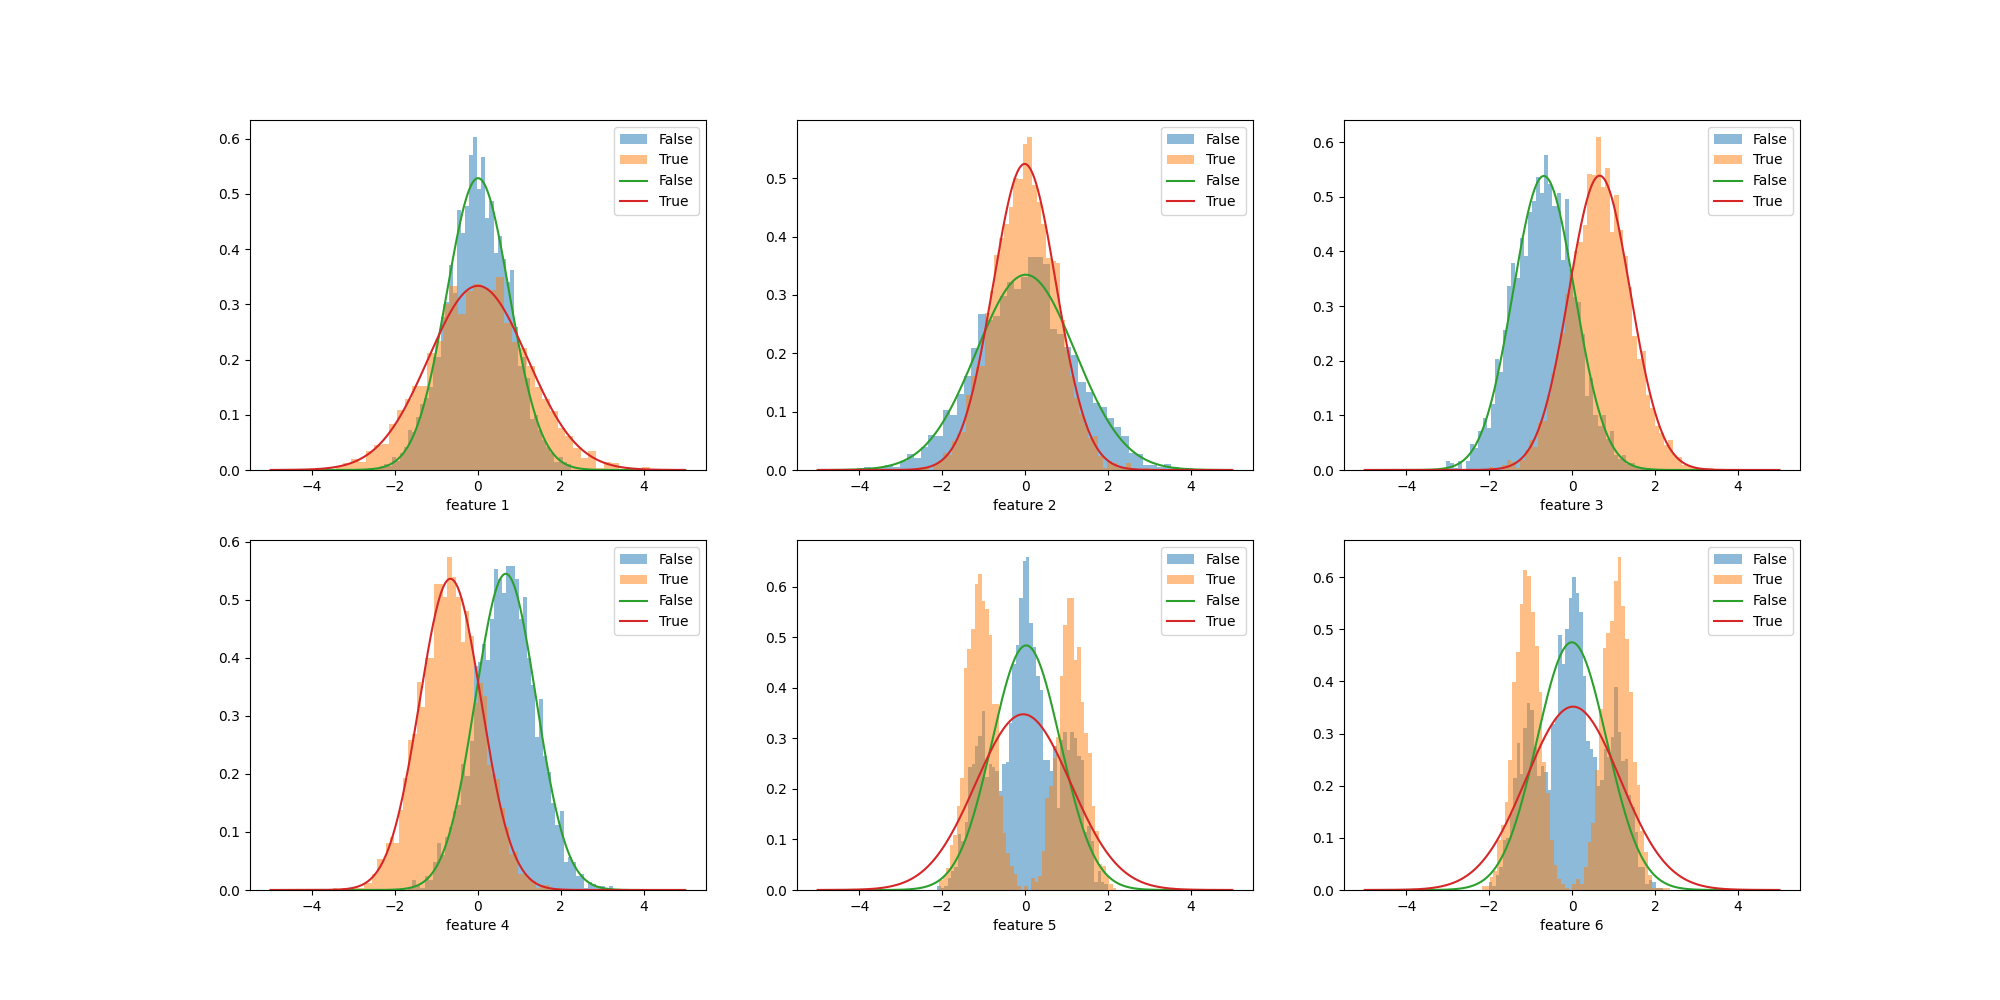
\includegraphics[width=1\linewidth]{Lab/04. Lab 04/Images/01. GaussianDensity}
    \caption{Gaussian Density}
    \label{fig:gaussianDensity}
\end{figure}

Thus, applying Gaussian probability density to the 6 features in our dataset, the following results in \autoref{fig:gaussianDensity},
are obteinded.\\
It can observe that \textbf{features 1 - 2 - 3 - 4} fit the Gaussian distribution,  the histogram of the data is well
approximated by the Gaussian curve.
For \textbf{features 5 - 6} this does not happen and therefore could not be a good model.

%    Classification Models


    \section{Model evaluation for classification}
    \label{sec:modelEvalution}
    %! Author = anton
%! Date = 30/08/2024

To assess whether one model classifies correctly or it is better than another, it is important to introduce what
may be a unit of measurement.
In particular, the evaluation of a model is done using the \textbf{DCF (Detection Cost Function)}
or also called \textbf{empirical Bayes Risk}.
But before delving into this method of valuation, we must consider what is called the working point
of a binary classification application.
This point is characterised by a triplet of values:

\begin{equation}
    \((\pi_T, C_{fn}, C_{fp})\)
    \label{eq:priorCfnCfp}
\end{equation}

where \(\pi_T\) is the prior probability of the target class, \(C_{fn}\) is the cost of a false negative and \(C_{fp}\) is the cost of a false positive.

But from \(\pi_T\), one can have attention on a particular triplet that is defined by:

\begin{equation}
    \((\tilde{\pi}, C_{fn}, C_{fp})\) = \((\tilde{\pi}, 1, 1)\)
    \label{eq:effecrivePriorCfnCfp}
\end{equation}

where \(\tilde{\pi}\) in \autoref{eq:effecrivePriorCfnCfp} is called \textbf{effective prior} probability of the target class, defined as:

\begin{equation}
    \tilde{\pi} = \frac{\pi_T C_{fn}}{\pi_T C_{fn} + (1 - \pi_T)C_{fp}}
    \label{eq:effectivePrior}
\end{equation}

So we can define \(DCF_u\) as:

\begin{equation}
    B_{emp} = DCF_u = \sum_{c=1}^{K} \frac{\pi_c}{N_c} \sum_{i\mid c_i = c} C(a(x_i, R)\mid c)
    \label{eq:empiricalBayesRisk}
\end{equation}

From \autoref{eq:empiricalBayesRisk}, we can obtain:

\begin{equation}
    DCF_u(\pi_T, C_{fn}, C_{fp}) = \pi_{T}C_{fn}P_{fn} + (1 - \pi_{T})C_{fp}P_{fp}
    \label{eq:DCFUnormalized}
\end{equation}

where:

\begin{equation}
    P_{fn} = \frac{FN}{FN + TP}\text{ ,}\quad
    P_{fp} = \frac{FP}{FP + TN}
    \label{eq:PfnPfp}
\end{equation}

From the \autoref{eq:empiricalBayesRisk}, it is possible to find \textbf{minDCF} and \textbf{actDCF}.
When calculating minDCF, the threshold used is the one that minimize DCF, and there are various methods for finding it.
Whereas for actDCF, the threshold used is:

\begin{equation}
    t' = - \log \frac{\tilde{\pi}}{1 - \tilde{\pi}}
    \label{eq:actDCFThreshold}
\end{equation}


    \section{Classification Models Analysis}
    \label{sec:classificationModels}
    %! Author = antonio
%! Date = 7/2/24

To perform the classification, the dataset must first be divided into two sub-portions, the training and validation sub-portions.

\subsection{Gaussian models}
\label{subsec:gaussianModels}
Since, it is dealing with a binary classification task, it will assign a probabilistic score to each sample in terms
of the class-posterior log-ratio:
\begin{equation}
    \log r(x_t) = \log \frac{P(C=h_1\mid x_t)}{P(C=h_0\mid x_t)}
    \label{eq:llr}
\end{equation}

Analysing \autoref{eq:llr} in more detail, it becomes:
\begin{equation}
    \log r(x_t) = \log \frac{f_{X\mid C}(x_t \mid h_1)}{f_{X\mid C}(x_t \mid h_0)} + \log \frac{P(C=h_1)}{P(C=h_0)}
    \label{eq:llrExpanded}
\end{equation}

The first addend of the equation is called the \textit{llr} or \textit{log-likelihood ratio} and an optimal decision is
given by \autoref{eq:llrDecision}.

\begin{equation}
    \log r(x_t) \gtrless 0
    \label{eq:llrDecision}
\end{equation}

Considering \(P(C=h_1) = \pi \) and \(P(C=h_0) = 1 - \pi\), from \autoref{eq:llrExpanded} and \autoref{eq:llrDecision},
it is possible to write that the class assignment is based on \autoref{eq:llrExpanded} and \autoref{eq:llrDecision},
to obtain \autoref{eq:assignmentClasses}.

\begin{equation}
    llr(x_t)=\log \frac{f_{X\mid C}(x_t \mid h_1)}{f_{X\mid C}(x_t \mid h_0)} \gtrless -\log \frac{\pi}{1 - \pi}
    \label{eq:assignmentClasses}
\end{equation}

%   Multivariate Gaussian Classifier

\subsubsection{Multivariate Gaussian Classifier}
\label{subsubsec:multivariateGaussianClassifier}
The first classifier is given by the empirical mean and covariance of each class,
\begin{equation}
    \mu_c^* = \frac{1}{N_c} \sum_{i\mid c_i=c} x_i\text{ ,}\quad
    \Sigma_c^* = \frac{1}{N_c} \sum_{i\mid c_i=c} (x_i - \mu_c^*)(x_i - \mu_c^*)^T
    \label{eq:meanAndVarianceMVG}
\end{equation}

%   Naive Bayes Gaussian Classifier

\subsubsection{Naive Bayes Gaussian Classifier}
\label{subsubsec:naiveBayesGaussianClassifier}
This model makes an important assumption that simplifies the number of parameters to be estimated,
it assumes that the features are indepenent given their class.
This causes the covariance matrix to be a diagonal matrix, consequently, matching MVG with the diagonal covariance matrix.
However, the assumption of independence may be too restrictive and lead to inferior performance if the features are indeed correlated.

\begin{equation}
    \mu_{c,[j]}^* = \frac{1}{N_c} \sum_{i\mid c_i = c} x_{i,[j]}\text{ ,}\quad
    \sigma_{c,[j]}^2 = \frac{1}{N_c} \sum_{i\mid c_i = c} (x_{i,[j]} - \mu_{c,[j]}^*)^2
    \label{eq:meanAndVarianceNBG}
\end{equation}

%   Tied Covariance Gaussian Classifier

\subsubsection{Tied Covariance Gaussian Classifier}
\label{subsubsec:tiedCovarianceGaussianClassifier}
The assumption of the latter model consists of its own average for each class, but an equal covariance matrix for all classes.

\begin{equation}
    \mu_c^* = \frac{1}{N_c} \sum_{i\mid c_i=c} x_i\text{ ,}\quad
    \Sigma^* = \frac{1}{N} \sum_{c} \sum_{i\mid c_i = c} (x_{i} - \mu_c)(x_{i} - \mu_c)^T
    \label{eq:tiedCovariance}
\end{equation}

\subsubsection{Gaussian Models Comparison}
\label{subsubsec:gaussianModelsComparison}

    % Lab 06 NO PROJECT PART

%   Performance of Classifier
    %! Author = anton
%! Date = 28/08/2024

Starting with the previous performance, it may be interesting to analyse how performance changes as three main
parameters vary:
\begin{itemize}
    \item \(\tilde{\pi}\): represents prior probability of the positive class
    \item \(C_{fn}\): misclassification cost of a sample predicted as negative but it is positive
    \item \(C_{fp}\): misclassification cost of a sample predicted as positive but it is negative
\end{itemize}

\begin{table}[h]
    \centering
    \begin{tabular}{>{\centering\arraybackslash}p{2.9cm} >{\centering\arraybackslash}p{2.9cm} >{\centering\arraybackslash}p{2.9cm} >{\centering\arraybackslash}p{2.9cm}}
        \toprule
        & \textbf{MVG} & \textbf{Naive Bayes} & \textbf{Tied Covariance} \\
        \midrule
        \multicolumn{4}{c}{\textbf{Application \((\tilde{\pi},C_{fn}, C_{fp}) = (0.5, 1, 1)\)}} \\
        \midrule
        \textbf{actDCF} & 0.1399       & 0.1439               & 0.1860                   \\
        \textbf{minDCF} & 0.1302       & 0.1311               & 0.1812                   \\
        \midrule
        \multicolumn{4}{c}{\textbf{Application \((\tilde{\pi},C_{fn}, C_{fp}) = (0.9, 1, 1)\)}} \\
        \midrule
        \textbf{actDCF} & 0.4001       & 0.3893               & 0.4626                   \\
        \textbf{minDCF} & 0.3423       & 0.3509               & 0.4421                   \\
        \midrule
        \multicolumn{4}{c}{\textbf{Application \((\tilde{\pi},C_{fn}, C_{fp}) = (0.1, 1, 1)\)}} \\
        \midrule
        \textbf{actDCF} & 0.3051       & 0.3022               & 0.4061                   \\
        \textbf{minDCF} & 0.2629       & 0.2569               & 0.3628                   \\
        \midrule
        \multicolumn{4}{c}{\textbf{Application \((\tilde{\pi},C_{fn}, C_{fp}) = (0.5, 1, 9)\)}} \\
        \midrule
        \textbf{actDCF} & 0.3051       & 0.3022               & 0.4061                   \\
        \textbf{minDCF} & 0.2629       & 0.2569               & 0.3628                   \\
        \midrule
        \multicolumn{4}{c}{\textbf{Application \((\tilde{\pi},C_{fn}, C_{fp}) = (0.5, 9, 1)\)}} \\
        \midrule
        \textbf{actDCF} & 0.4001       & 0.3893               & 0.4626                   \\
        \textbf{minDCF} & 0.3423       & 0.3509               & 0.4421                   \\
        \bottomrule
    \end{tabular}
    \captionsetup{justification=justified,singlelinecheck=false,format=hang}
    \caption{Table showing minDCF and actDCF for different models and applications.}
    \label{tab:resultPerformanceClassifierWithoutPCA}
\end{table}

Analysing the results of the \autoref{tab:resultPerformanceClassifierWithoutPCA}, it is possible to observe:

\begin{table}[h]
    \centering
    \begin{tabular}{>{\centering\arraybackslash}p{2.9cm} >{\centering\arraybackslash}p{2.9cm} >{\centering\arraybackslash}p{2.9cm} >{\centering\arraybackslash}p{2.9cm}}
        \toprule
        & \textbf{MVG} & \textbf{Naive Bayes} & \textbf{Tied Covariance} \\
        \toprule
        \toprule
        \multicolumn{4}{c}{\textbf{Application \((\tilde{\pi},C_{fn}, C_{fp}) = (0.5, 1, 1)\)}} \\
        \midrule
        \multicolumn{4}{c}{\textbf{no PCA}} \\
        \midrule
        \textbf{actDCF} & 0.1399       & 0.1439               & 0.1860                   \\
        \textbf{minDCF} & 0.1302       & 0.1311               & 0.1812                   \\
        \midrule
        \multicolumn{4}{c}{\textbf{PCA}} \\
        \multicolumn{4}{c}{\textbf{\(m = 5\)}} \\
        \midrule
        \textbf{actDCF} & 0.1419       & 0.1749               & 0.1860                   \\
        \textbf{minDCF} & 0.1331       & 0.1737               & 0.1812                   \\
        \midrule
        \multicolumn{4}{c}{\textbf{\(m = 6\)}} \\
        \midrule
        \textbf{actDCF} & 0.1399       & 0.1780               & 0.1860                   \\
        \textbf{minDCF} & 0.1302       & 0.1727               & 0.1812                   \\
        \toprule
        \toprule
        \multicolumn{4}{c}{\textbf{Application \((\tilde{\pi},C_{fn}, C_{fp}) = (0.9, 1, 1)\)}} \\
        \midrule
        \multicolumn{4}{c}{\textbf{no PCA}} \\
        \midrule
        \textbf{actDCF} & 0.4001       & 0.3893               & 0.4626                   \\
        \textbf{minDCF} & 0.3423       & 0.3509               & 0.4421                   \\
        \midrule
        \multicolumn{4}{c}{\textbf{PCA}} \\
        \multicolumn{4}{c}{\textbf{\(m = 5\)}} \\
        \midrule
        \textbf{actDCF} & 0.3980       & 0.4660               & 0.4626                   \\
        \textbf{minDCF} & 0.3512       & 0.4340               & 0.4451                   \\
        \midrule
        \multicolumn{4}{c}{\textbf{\(m = 6\)}} \\
        \midrule
        \textbf{actDCF} & 0.4001       & 0.4512               & 0.4626                   \\
        \textbf{minDCF} & 0.3423       & 0.4359               & 0.4421                   \\
        \toprule
        \toprule
        \multicolumn{4}{c}{\textbf{Application \((\tilde{\pi},C_{fn}, C_{fp}) = (0.1, 1, 1)\)}} \\
        \midrule
        \multicolumn{4}{c}{\textbf{no PCA}} \\
        \midrule
        \textbf{actDCF} & 0.3051       & 0.3022               & 0.4061                   \\
        \textbf{minDCF} & 0.2629       & 0.2569               & 0.3628                   \\
        \midrule
        \multicolumn{4}{c}{\textbf{PCA}} \\
        \multicolumn{4}{c}{\textbf{\(m = 5\)}} \\
        \midrule
        \textbf{actDCF} & 0.3042       & 0.3930               & 0.4051                   \\
        \textbf{minDCF} & 0.2738       & 0.3545               & 0.3648                   \\
        \midrule
        \multicolumn{4}{c}{\textbf{\(m = 6\)}} \\
        \midrule
        \textbf{actDCF} & 0.3051       & 0.3920               & 0.4061                   \\
        \textbf{minDCF} & 0.2629       & 0.3535               & 0.3628                   \\
        \bottomrule
    \end{tabular}
    \captionsetup{justification=justified,singlelinecheck=false,format=hang}
    \caption{Show minDCF and actDCF for different models and applications before and after applying PCA.}
    \label{tab:resultPerformanceClassifierWithPCA}
\end{table}

\begin{figure}[h!]
    \centering
    \begin{subfigure}[b]{0.4\linewidth}
        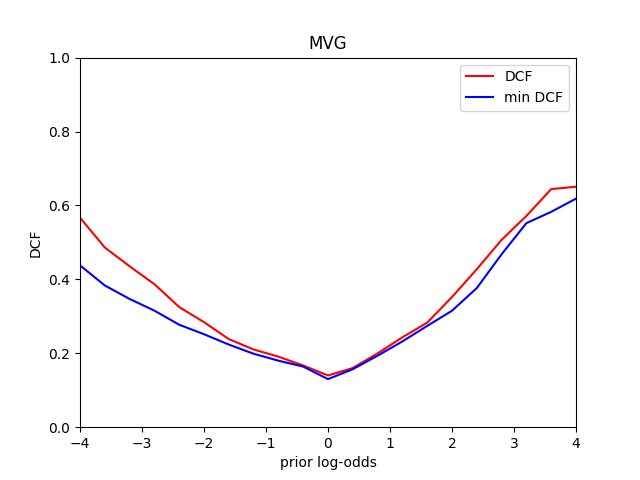
\includegraphics[width=\linewidth]{Lab/07. Lab 07/Images/01. MVG}
        \caption{Without mean}
        \label{fig:dcfMVG}
    \end{subfigure}
    \begin{subfigure}[b]{0.4\linewidth}
        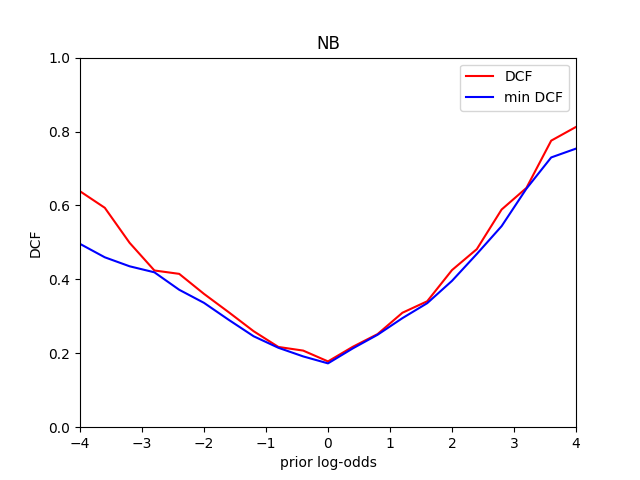
\includegraphics[width=\linewidth]{Lab/07. Lab 07/Images/02. Naive Bayes}
        \caption{With mean}
        \label{fig:dcfNB}
    \end{subfigure}
    \begin{subfigure}[b]{0.4\linewidth}
        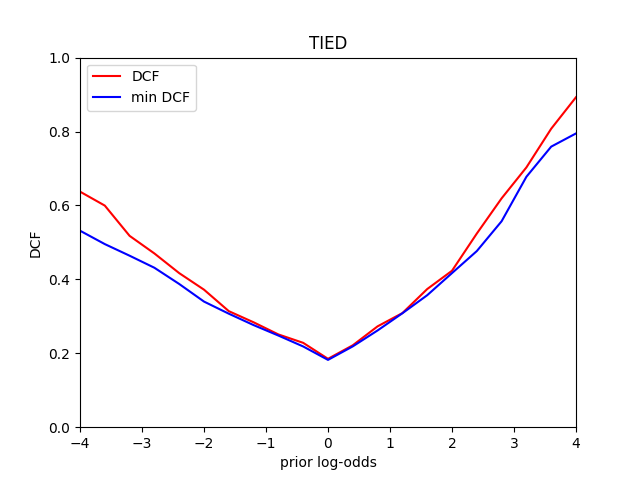
\includegraphics[width=\linewidth]{Lab/07. Lab 07/Images/03. Tied}
        \caption{With mean}
        \label{fig:dcfTC}
    \end{subfigure}
    \caption{}
    \label{fig:dcfMVGNBTC}
\end{figure}

%   Logistic Regression Classifier

    \subsection{Logistic Regression Classifier}
    \label{subsec:logisticRegressionClassifier}
    %! Author = antonio
%! Date = 7/2/24

Logistic Regression is a discriminative classification model, directly evaluating the posterior probability \(C \mid X\).
In particular by determining that hyperplane which maximises the posterior probability.
Starting from the results obtained from the Tied Gaussian that provides log-likelihood ratios that are linear functions
of our data, where log-posterior probability ratio is:

\begin{equation}
    \log \frac{P(C=h_1 \mid X)}{P(C=h_0 \mid X)} = \log \frac{f_{X \mid C}(x \mid h_1)}{f_{X \mid C}(x \mid h_0)} + \log \frac{\pi}{1-\pi} = \omega^T x + b
    \label{eq:logisticRegression}
\end{equation}

where prior information has been absorbed in the bias term \(b\) of the \autoref{eq:logisticRegression}.
So from this point we can define the score function as:

\begin{equation}
    s(x) = \omega^T x + b = 0
    \label{eq:scoreFunctionLR}
\end{equation}

where it is positive for samples of class \(h_1\) and negative for samples of class \(h_0\).
Given \(\omega\) and \(b\) we can compute the posterior class probability as:

\begin{equation}
    P(C=h_1 \mid x, \omega, b) = \sigma(\omega^T x + b) = \sigma(s(x))
    \label{eq:posteriorClassProbabilityLR}
\end{equation}
where \(\sigma\) is sigmoid function defined as:

\begin{equation}
    \sigma(x) = \frac{1}{1 + e^{-x}}
\end{equation}

This approach assumes that the decision rules will be hyperplanes orthogonal to vector w.

\subsubsection{Binary Logistic Regression}
\textbf{Binary Logistic Regression Not Prior-Weighted}\par
The objective is to minimise the loss function \(J(\omega,b)\), but to this is introduced what is a penalty term,
so the new function becomes:

\begin{equation}
    J(\omega,b) = \frac{\lambda}{2}\left\|w \right\|^2 + \frac{1}{n} \sum_{i=1}^{n} \log (1+e^{-z_i(\omega^T x_i + b)}), \quad
    z_i = \begin{cases}
              1 & \text{if } c_i = 1 \\
              -1 & \text{if } c_i = 0
    \end{cases}
    \label{eq:minimiseFunctionLR}
\end{equation}

where \(\lambda\) of \autoref{eq:minimiseFunctionLR} is the regularization term, this term has been introduced to make problem
solvable in case of linearly separable classes.

\begin{figure}[h!]
    \centering
    \begin{subfigure}[b]{0.40\linewidth}
        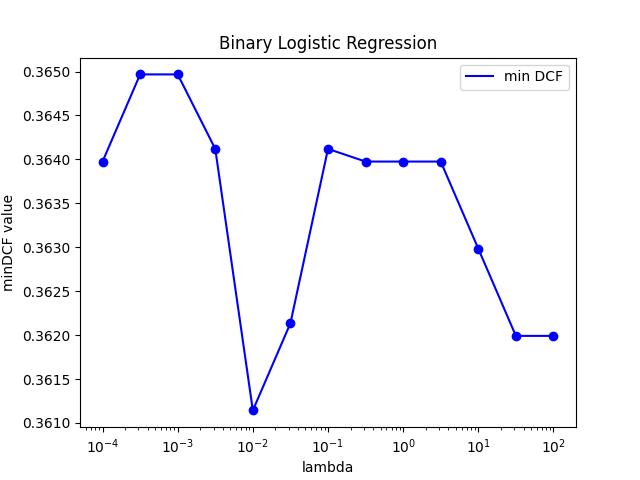
\includegraphics[width=\linewidth]{Lab/08. Lab 08/Images/01. BLR - minDCF}
        \label{fig:BLRminDCF}
    \end{subfigure}
    \begin{subfigure}[b]{0.40\linewidth}
        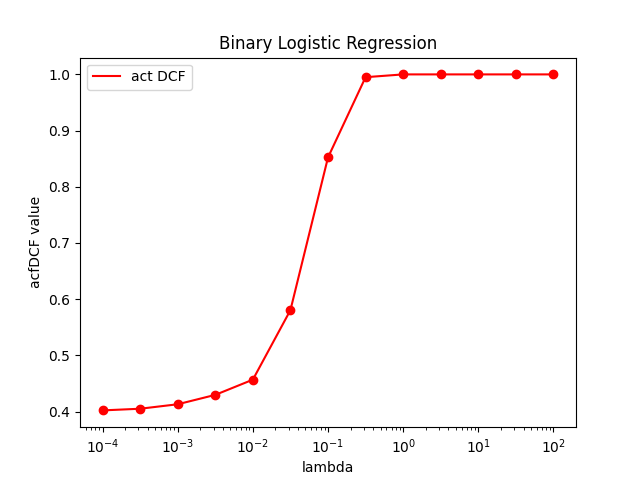
\includegraphics[width=\linewidth]{Lab/08. Lab 08/Images/02. BLR - actDCF}
        \label{fig:BLRactDCF}
    \end{subfigure}
    \begin{subfigure}[b]{0.40\linewidth}
        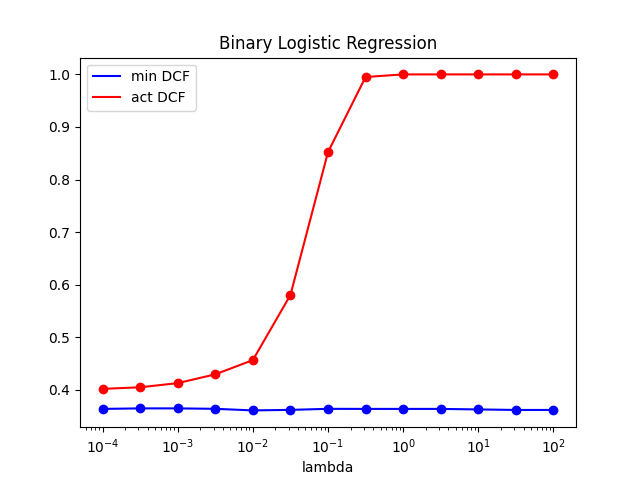
\includegraphics[width=\linewidth]{Lab/08. Lab 08/Images/03. BLR - min And actDCF}
        \label{fig:BLRminAndactDCF}
    \end{subfigure}
    \begin{subfigure}[b]{0.40\linewidth}
        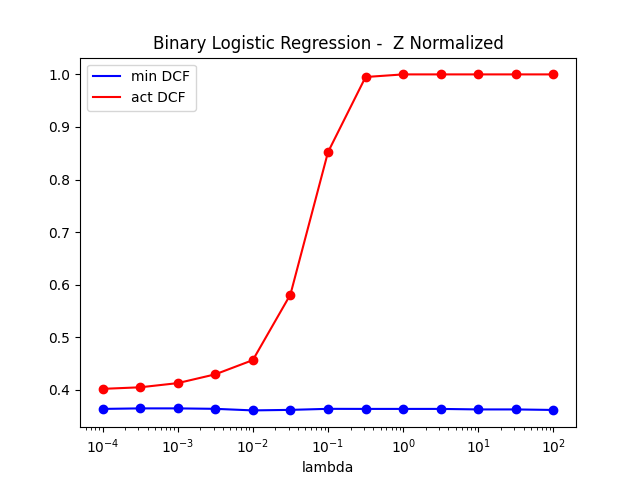
\includegraphics[width=\linewidth]{Lab/08. Lab 08/Images/04. BLR - minAnd actDCF - ZNormalized}
        \label{fig:BLRminAndactDCFZNorm}
    \end{subfigure}
    \caption{Binary Logistic Regression not Prior-Weighted}
    \label{fig:BLR}
\end{figure}

\begin{figure}[h!]
    \centering
    \begin{subfigure}[b]{0.40\linewidth}
        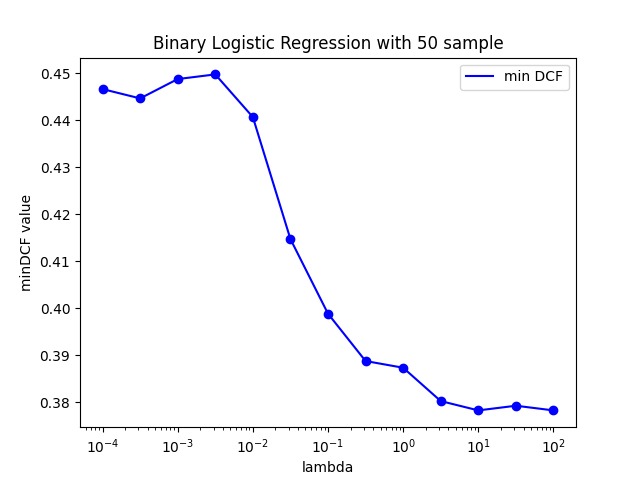
\includegraphics[width=\linewidth]{Lab/08. Lab 08/Images/05. BLR - minDCF 50 Samples}
        \label{fig:BLR50SminDCF}
    \end{subfigure}
    \begin{subfigure}[b]{0.40\linewidth}
        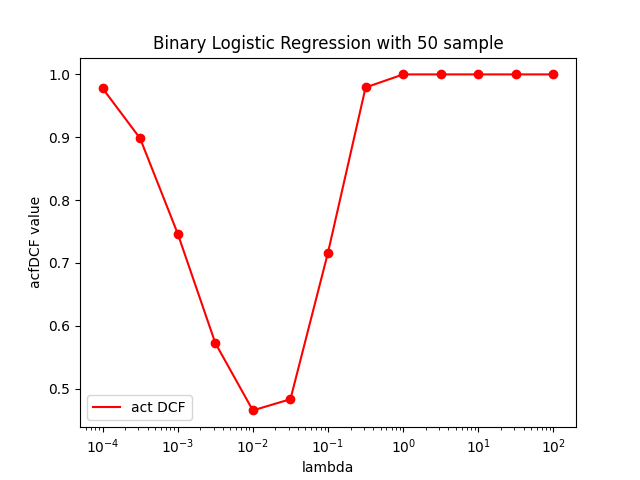
\includegraphics[width=\linewidth]{Lab/08. Lab 08/Images/06. BLR - actDCF 50 Samples}
        \label{fig:BLR50SactDCF}
    \end{subfigure}
    \begin{subfigure}[b]{0.40\linewidth}
        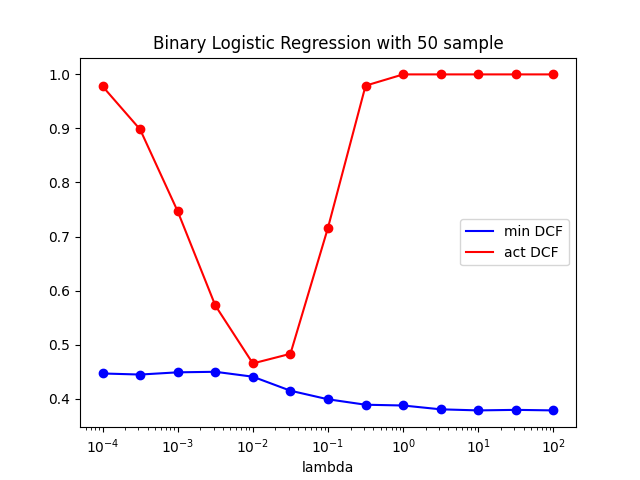
\includegraphics[width=\linewidth]{Lab/08. Lab 08/Images/07. BLR - minAndactDCF 50 Samples}
        \label{fig:BLR50SminAndactDCF}
    \end{subfigure}
    \begin{subfigure}[b]{0.40\linewidth}
        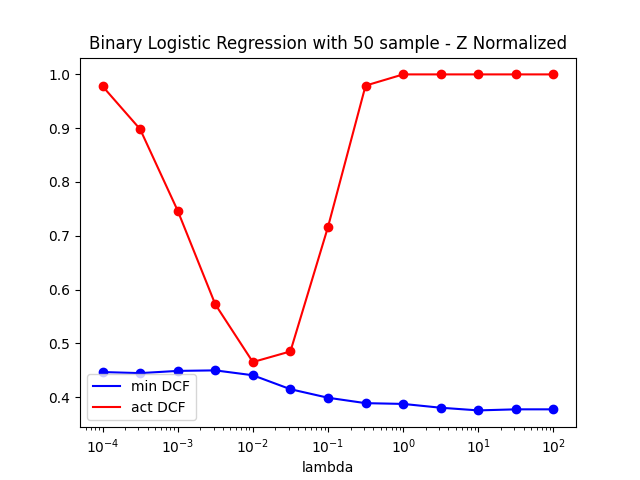
\includegraphics[width=\linewidth]{Lab/08. Lab 08/Images/08. BLR - minAndactDCF 50 Samples - ZNormalized}
        \label{fig:minAndactDCFZNorm}
    \end{subfigure}
    \caption{Binary Logistic Regression not Prior-Weighted with 50 Samples}
    \label{fig:BLR50Samples}
\end{figure}

In this model \(\pi_T = 0.1\) is used.
In \autoref{tab:minDCFactDCFBLRNPW}, it can be seen how the values of minDCF and actDCF vary when \(\lambda\) changes,
Z-normalization is applied or not and if the whole training set or a portion was used.
It can be deduced from the values obtained that the application of z-normalisation brings no advantage.
On the other hand, by using only 50 samples, it can see that using a limited number of samples can significantly
influence the model and could lead to misleading results that are not representative of the entire sample.
Consequently, as many samples as possible should be used for training to obtain a more accurate model.
\autoref{fig:BLR} and \autoref{fig:BLR50Samples} give a graphic representation of how minDCF and actDCF vary with \(\lambda\)

\begin{table}[h!]
    \centering
    \begin{tabular}{>{\centering\arraybackslash}p{2cm} >{\centering\arraybackslash}p{2cm} >{\centering\arraybackslash}p{2cm} >{\centering\arraybackslash}p{2cm}>{\centering\arraybackslash}p{2cm}}
        \toprule
        \multicolumn{5}{c}{\textbf{Binary Logistic Regression Not Prior-Weighted}} \\
        \midrule
        \multirow{2}{*}{\centering \textbf{\(\lambda\)}} & \multicolumn{2}{c}{\textbf{minDCF}} & \multicolumn{2}{c}{\textbf{actDCF}} \\
        \cmidrule(lr){2-5}
        & \textbf{no z-norm} & \textbf{z-norm} & \textbf{no z-norm} & \textbf{z-norm} \\
        \midrule
        \(10^{-4}\) & 0.3640             & 0.3640          & 0.4021             & 0.4021          \\
        \(10^{-3}\) & 0.3650             & 0.3650          & 0.4130             & 0.4130          \\
        \(10^{-2}\) & 0.3611             & 0.3611          & 0.4568             & 0.4568          \\
        \(10^{-1}\) & 0.3641             & 0.3641          & 0.8522             & 0.8522          \\
        \midrule
        \midrule
        \multicolumn{5}{c}{\textbf{Binary Logistic Regression Not Prior-Weighted (50 Samples)}} \\
        \midrule
        \multirow{2}{*}{\centering \textbf{\(\lambda\)}} & \multicolumn{2}{c}{\textbf{minDCF}} & \multicolumn{2}{c}{\textbf{actDCF}} \\
        \cmidrule(lr){2-5}
        & \textbf{no z-norm} & \textbf{z-norm} & \textbf{no z-norm} & \textbf{z-norm} \\
        \midrule
        \(10^{-4}\) & 0.4466             & 0.4466          & 0.9780             & 0.9780          \\
        \(10^{-3}\) & 0.4487             & 0.4487          & 0.7466             & 0.7466          \\
        \(10^{-2}\) & 0.4407             & 0.4407          & 0.4652             & 0.4652          \\
        \(10^{-1}\) & 0.3988             & 0.3988          & 0.7164             & 0.7164          \\
        \bottomrule
    \end{tabular}
    \captionsetup{justification=justified,singlelinecheck=false,format=hang}
    \caption{Show minDCF and actDCF for Binary Logistic Regression Not Prior-Weighted model}
    \label{tab:minDCFactDCFBLRNPW}
\end{table}

\newpage
\textbf{Binary Logistic Regression Prior-Weighted}\par
Another possible Logistic Regression approach is that Prior-Weighted; it allows to simulate different priors for class 1.
Therefore, the objective function becomes:

\begin{equation}
    J(\omega,b) = \frac{\lambda}{2}\left\|w \right\|^2 + \sum_{i=1}^{n} \xi_i\log (1+e^{-z_i(\omega^T x_i + b)}),\quad
    \xi_i = \begin{cases}
                \frac{\pi_t}{n_T} & \text{if } z_i = +1 (c_i = 1) \\
                \frac{1 - \pi_T}{n_F} & \text{if } z_i = -1 (c_i = 0) \\
    \end{cases}
    \label{eq:minimiseFunctionLRPW}
\end{equation}

Now it is possible analyze the results obtained from the Prior-Weighted model with \(\pi_T = 0.1\).

\begin{figure}[h!]
    \centering
    \begin{subfigure}[b]{0.30\linewidth}
        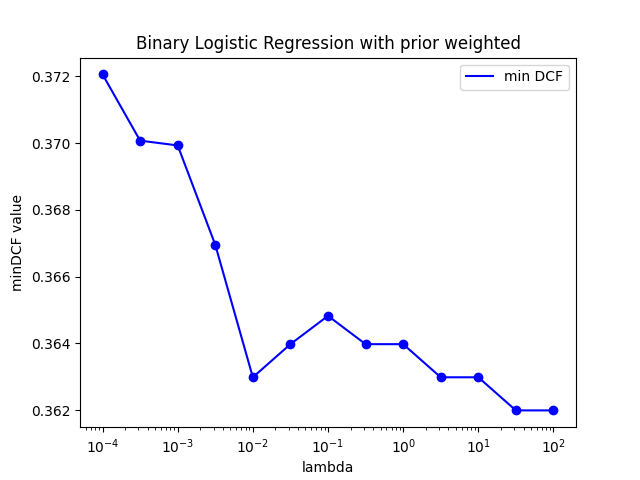
\includegraphics[width=\linewidth]{Lab/08. Lab 08/Images/09. PW - minDCF}
        \label{fig:PWminDCF}
    \end{subfigure}
    \begin{subfigure}[b]{0.30\linewidth}
        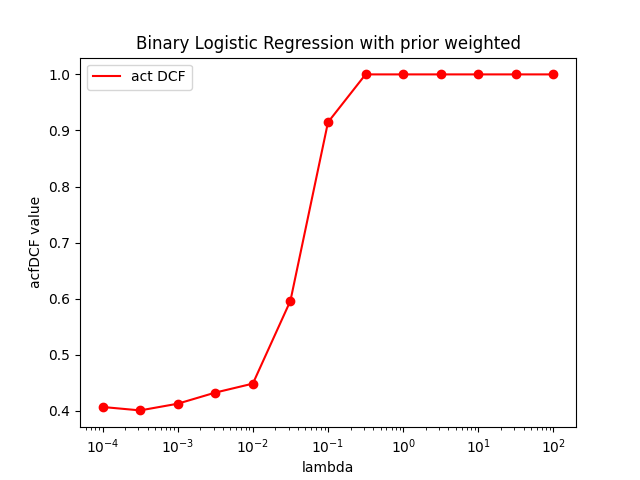
\includegraphics[width=\linewidth]{Lab/08. Lab 08/Images/10. PW - actDCF}
        \label{fig:PWactDCF}
    \end{subfigure}
    \begin{subfigure}[b]{0.30\linewidth}
        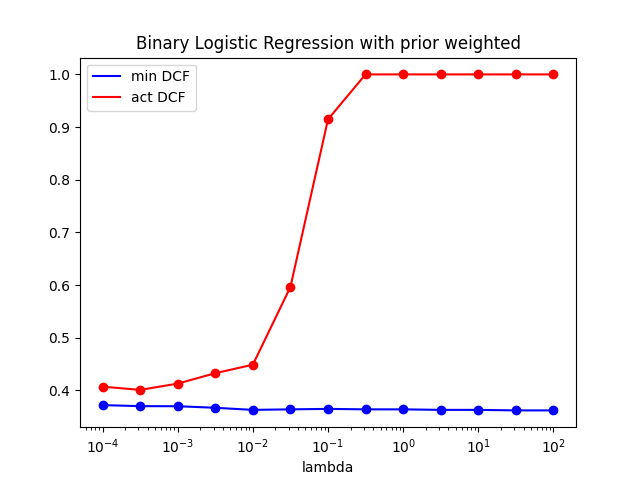
\includegraphics[width=\linewidth]{Lab/08. Lab 08/Images/11. PW - minAndActDCF}
        \label{fig:PWminAndactDCF}
    \end{subfigure}
    \caption{Binary Logistic Regression Prior-Weighted}
    \label{fig:PW}
\end{figure}

\begin{table}[h!]
    \centering
    \begin{tabular}{>{\centering\arraybackslash}p{2cm} >{\centering\arraybackslash}p{2cm} >{\centering\arraybackslash}p{2cm}}
        \toprule
        \multicolumn{3}{c}{\textbf{Binary Logistic Regression Prior-Weighted }} \\
        \midrule
        \multicolumn{3}{c}{\(\pi_T = 0.1 \)} \\
        \midrule
        \textbf{\(\lambda\)} & \textbf{minDCF} & \textbf{actDCF} \\
        \midrule
        \(10^{-4}\)          & 0.3721          & 0.4071          \\
        \(10^{-3}\)          & 0.3699          & 0.4129          \\
        \(10^{-2}\)          & 0.3630          & 0.4487          \\
        \(10^{-1}\)          & 0.3648          & 0.9147          \\
        \bottomrule
    \end{tabular}
    \captionsetup{justification=justified,singlelinecheck=false,format=hang}
    \caption{Show minDCF and actDCF for Binary Logistic Regression Prior-Weighted}
    \label{tab:minDCFactDCFPW}
\end{table}

The role of the prior is to weight the samples during model training.
In particular, samples in the higher priority class receive a higher weight than those in the lower priority class.
This can be useful if the dataset is unbalanced, the choice of the prior must be made at the beginning and this choice
can affect the model a lot, in fact we may even have a worsening of the model. \\
Comparing the results obtained in \autoref{tab:minDCFactDCFBLRNPW} and \autoref{tab:minDCFactDCFPW},
there isn't noticeable change in the outcomes on minDCF and actDCF this means that our dataset is not unbalanced.
The interesting value to observe is the value of actDCF when \(\lambda= 10^-1\).\\

\textbf{Binary Logistic Regression with Pre-processing (PCA)}\par
In this case, PCA can be applied as pre-processing, and by looking at the values in \autoref{tab:minDCFactDCFBLPCA},
it can be seen that it does not result much improvement of the system.

\begin{figure}[h!]
    \centering
    \begin{subfigure}[b]{0.30\linewidth}
        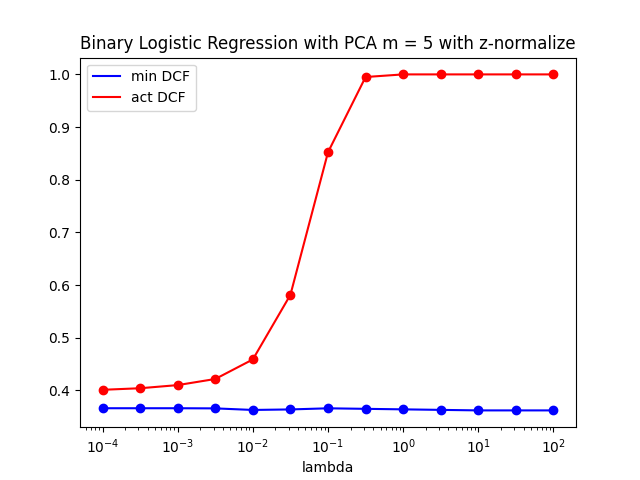
\includegraphics[width=\linewidth]{Lab/08. Lab 08/Images/12. BLR - PCA m=5 Z-norm}
        \label{fig:BLRPCAm5ZNorm}
    \end{subfigure}
    \begin{subfigure}[b]{0.30\linewidth}
        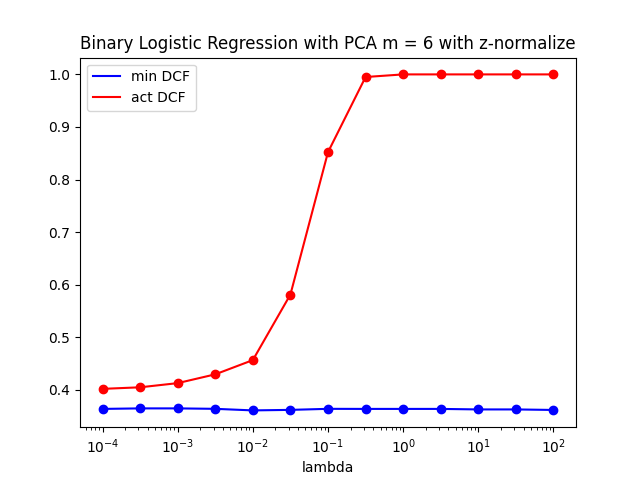
\includegraphics[width=\linewidth]{Lab/08. Lab 08/Images/13. BLR - PCA m=6 Z-norm}
        \label{fig:BLRPCAm6ZNorm}
    \end{subfigure}
    \caption{Binary Logistic Regression applying PCA and z-normalization}
    \label{fig:BLRPCA}
\end{figure}

\begin{table}[h!]
    \centering
    \begin{tabular}{>{\centering\arraybackslash}p{2cm} >{\centering\arraybackslash}p{2cm} >{\centering\arraybackslash}p{2cm}>{\centering\arraybackslash}p{2cm}>{\centering\arraybackslash}p{2cm}}
        \toprule
        \multicolumn{5}{c}{\textbf{Binary Logistic Regression with PCA }} \\
        \midrule
        \multirow{2}{*}{\centering \textbf{\(\lambda\)}} & \multicolumn{2}{c}{\textbf{minDCF}} & \multicolumn{2}{c}{\textbf{actDCF}} \\
        \cmidrule(lr){2-5}
        & \textbf{no z-norm} & \textbf{z-norm} & \textbf{no z-norm} & \textbf{z-norm} \\
        \midrule
        \multicolumn{5}{c}{\textbf{\(m=5\)}} \\
        \midrule
        \(10^{-4}\) & 0.3661             & 0.3661          & 0.4011             & 0.4011          \\
        \(10^{-3}\) & 0.3661             & 0.3661          & 0.4100             & 0.4100          \\
        \(10^{-2}\) & 0.3618             & 0.3628          & 0.4578             & 0.4588          \\
        \(10^{-1}\) & 0.3660             & 0.3660          & 0.8502             & 0.8522          \\
        \midrule
        \multicolumn{5}{c}{\textbf{\(m=6\)}} \\
        \midrule
        \(10^{-4}\) & 0.3640             & 0.3640          & 0.4021             & 0.4021          \\
        \(10^{-3}\) & 0.3650             & 0.3650          & 0.4130             & 0.4130          \\
        \(10^{-2}\) & 0.3611             & 0.3611          & 0.4568             & 0.4568          \\
        \(10^{-1}\) & 0.3641             & 0.3641          & 0.8522             & 0.8522          \\
        \bottomrule
    \end{tabular}
    \captionsetup{justification=justified,singlelinecheck=false,format=hang}
    \caption{Show minDCF and actDCF for Binary Logistic Regression applying PCA and with adn withoud z-normalization}
    \label{tab:minDCFactDCFBLPCA}
\end{table}


%\subsubsection{Quadratic Logistic Regression}
%In this step we can analyze training on a Quadratic Logistic Regression model by performing features expansion, so it's possible write log-likelihood ratio as:
%\begin{equation}
%    \log{\frac{P(C=h_1|x)}{P(C=h_0|x)}}=x^TAx+b^Tx+c=s(\textbf{x},\textbf{A},\textbf{b},\textbf{c})
%\end{equation}
%This expression is quadratic in x but it's linear in A and b.
%We could rewrite it to obtain a decision function that is linear for the expanded features space but quadratic in original features space.\\
%We can write features expansion as:
%\begin{equation}
%    \Phi(x)=
%    \begin{bmatrix}
%        vec(xx^T) \\
%        x
%    \end{bmatrix},
%    \;\;
%    w=
%    \begin{bmatrix}
%        vec(A) \\
%        b
%    \end{bmatrix}
%\end{equation}
%where vec(X) is the operator that stacks the columns of X into a single column vector. In this way we can write the posterio log-likelihood as:
%\begin{equation}
%    s(x,w,c)=s^T\phi(x)+c
%\end{equation}
%
%Tabella
%
%In conclusion, the results obtained from the Quadratic Logistic Regression model show that

%   Support Vector Machine Classifier

    \subsection{Support Vector Machine Classifier}
    \label{subsec:supportVectorMachineClassifier}
    %! Author = antonio
%! Date = 7/2/24

\subsubsection{Linear Support Vector Machines}
Support Vector Machines are linear classifiers that look for maximum margin separation hyperplanes. The primal formulation of the soft-margin SVM problem consists in minimizing the function:
\begin{equation}
    \mathbf{J}(w,b)= \frac{1}{2}||w||^2 + C\sum_{i=1}^{N}max(0,1-z_i(w^Tx_i+b))
\end{equation}
where N is the number of training samples, C is the regularization parameter, and \(z_i\) is the margin of the i-th sample.\\
The dual formulation of the problem is:
\begin{equation}
    \mathbf{J}(\alpha)= - \frac{1}{2} \alpha^T \;\textbf{H} \;\alpha + \alpha^T \textbf{1} \;\;\;\;\;\;1\leq \alpha_i\leq C,\;\; \forall i \in \{1,...,N\},\;\; \sum_{i=1}^{n}\alpha_i z_i=0
\end{equation}
where H is \(H_{ij}=z_iz_jx_i^Tx_j\) and the dual solution is the maximizer of \(J^D(\alpha)\).\\
Primal and dual solutions are releted through:
\begin{equation}
    w^*=\sum_{i=1}^{N}\alpha_i^* z_i x_i
\end{equation}
In addition it's possible to rewrite dual problem as minimization of:
\begin{equation}
   \hat{\mathbf{L}}(\alpha)=-\mathbf{J}(\alpha)= \frac{1}{2} \alpha^T \;\textbf{H} \;\alpha - \alpha^T \textbf{1}
\end{equation}
and it can be minimize by L-BFGS-B algorithm.
After that we have calculated the optimal \(\alpha\) we can compute \(w^*\).

\subsubsection{Kernel Support Vector Machines}
It's possible in Support Vector Machines to use kernels to allow nonlinear classification.
In this case there is no explicit expansion of the feature space; 
we only can calculate the scalar product between the expanded features:\( k(x_1,x_2)=\phi(x_1)_T\phi(x_2)\) where k is the kernel function.
To do this we need to go and replace H as we saw in the previous section with \(\hat{H}= z_iz_jk(x_1,x_2)\). 
During our project we see two different types of kernels:
\begin{itemize}
    \item \textbf{Polynomial kernel of degree d}: \(k(x_1,x_2)=(x_1^Tx_2+c)^d\)
    \item \textbf{Radial Basis Function kernel(RBF)}: \(k(x_1,x_2)=e^{-\gamma||x1-x_2||^2}\)
\end{itemize}
We can now apply the polynomial kernel to the SVM with \(d=2,\;\; c=1, \;\;\xi=0\) and see how minDCF and actDCF vary as C changes.


tabelle e conclusioni


%   Gaussian Mixtures Models

    \subsection{Gaussian Mixture Models Classifier}
    \label{subsec:gaussianMixtureModels}
    %! Author = antonio
%! Date = 7/2/24
The last model we are going to consider is a generative model, the Gaussian Mixture Model (GMM).
This model is based on the assumption that the data is generated by a mixture of K Gaussian distributions.
The GMM density consists of a weighted sum of K Gaussians:

\begin{equation}
    \mathbf{X}\thicksim  GMM(\mathbf{M} ,\mathcal{S},w)\implies f_x(x)=\sum_{c=1}^{K}\mathcal{N}(x|\mu_g,\Sigma_g)w_g
    \label{eq:GMM}
\end{equation}

where \( M=[\mu_1...\mu_k]\), \(\mathcal{S}=[\Sigma_1...\Sigma_k]\) and \(w=[w_1...w_k]\) of \autoref{eq:GMM} are the parameters of the model.\\
Gaussian components can be viewed as clusters to which the samples belong (hard or soft), and the cluster label is an unobserved latent random variable.
We can also define in this case the responsability term, defined as \autoref{eq:responsability}, that represents the
posterior probability that a sample belongs to a certain cluster:

\begin{equation}
    \gamma(z_{n,i})=P(G_i=g| X_i=x)=\frac{f_{x_i,G_i}(x_i,g)}{f_{x_i}(x_i)}=\frac{\mathcal{N}(x_i|\mu_g,\Sigma_g)w_g}{\sum_{g'}\mathcal{N}(x_i|\mu_{g'},\Sigma_{g'})w_{g'}}
    \label{eq:responsability}
\end{equation}

Then assign the sample to the cluster label for which the responsability is highest and re-estimate the model parameters based on the cluster assignment.
We can apply the Expectation-Maximization algorithm to estimate the model parameters.
The EM algorithm is an iterative algorithm that consists of two steps:
\begin{itemize}
    \item Expectation stage: estimation of the responsability (given the model parameters \((M_t,S_t,w_t)\))
    \item Maximization step: estimation of new model parameters using the above statistics, estimation continues from an
    initial value of the model parameters until a certain criterion is met.
\end{itemize}

The EM algorithm then requires an initial estimate for the GMM parameters, so we use the LBG algorithm to incrementally construct a
GMM with 2G components from a GMM with G components.
The starting point will be \( (1,\mu,\sigma)\), so we use the empirical mean and covariance matrix of the data set.
Then it builds a 2-component model starting from one and from each of the new components 2 more components are generated and so on.
GMM can have differents versions as:
\begin{itemize}
    \item \textbf{The full covariance model:} in this case each component has a full covariance matrix, which means that all possible covariances between the variables are considered.
    \item \textbf{The diagonal covariance model:} in this setup, the covariance matrix of each component is assumed to be diagonal, which means the variables are considered independent.
\end{itemize}

As an initial point in our project, we considered having a maximum component number of 32 and using the two methods mentioned above.
So at first we evaluated the model where the number of components for class 0 and class 1 were equal, obtaining the results shown in
\autoref{tab:GMMSameComponents}.

\begin{table}[h!]
    \centering
    \begin{tabular}{>{\centering\arraybackslash}p{2cm} >{\centering\arraybackslash}p{2cm} >{\centering\arraybackslash}p{2cm} >{\centering\arraybackslash}p{2cm} >{\centering\arraybackslash}p{2cm}}
        \toprule
        \multicolumn{5}{c}{\textbf{GMM Model}} \\
        \midrule
        \multirow{2}{*}{\textbf{(nc0, nc1)}} & \multicolumn{2}{c}{\textbf{Full Cov}} & \multicolumn{2}{c}{\textbf{Diag Cov}} \\
        \cmidrule(lr){2-5}
        & \textbf{minDCF} & \textbf{actDCF} & \textbf{minDCF} & \textbf{actDCF} \\
        \midrule
        (1, 1)   & 0.2629          & 0.3051          & 0.2570          & 0.3022          \\
        (2, 2)   & 0.2170          & 0.2337          & 0.2489          & 0.2674          \\
        (4, 4)   & 0.2161          & 0.2395          & 0.1481          & 0.1687          \\
        (8, 8)   & 0.1786          & 0.1928          & 0.1463          & 0.1809          \\
        (16, 16) & 0.1631          & 0.1766          & 0.1622          & 0.1769          \\
        (32, 32) & 0.2337          & 0.2499          & 0.1766          & 0.1989          \\
        \bottomrule
    \end{tabular}
    \captionsetup{justification=justified,singlelinecheck=false,format=hang}
    \caption{Show minDCF and actDCF for same number of components in GMM}
    \label{tab:GMMSameComponents}
\end{table}

Subsequently, all possible combinations within the maximum value indicated above were tested.
\autoref{tab:GMMBestComponents} shows what may be the most significant values.
I chose these combinations because (1,16) and (2,16) are the two best combinations for the Full Covariance method,
whereas (8,32) and (8,16) are the best for Diagonal Covariance method.

\begin{table}[h!]
    \centering
    \begin{tabular}{>{\centering\arraybackslash}p{2cm} >{\centering\arraybackslash}p{2cm} >{\centering\arraybackslash}p{2cm} >{\centering\arraybackslash}p{2cm} >{\centering\arraybackslash}p{2cm}}
        \toprule
        \multicolumn{5}{c}{\textbf{GMM Model}} \\
        \midrule
        \multirow{2}{*}{\textbf{(nc0, nc1)}} & \multicolumn{2}{c}{\textbf{Full Cov}} & \multicolumn{2}{c}{\textbf{Diag Cov}} \\
        \cmidrule(lr){2-5}
        & \textbf{minDCF} & \textbf{actDCF} & \textbf{minDCF} & \textbf{actDCF} \\
        \midrule
        (1, 16) & 0.1495          & 0.2055          & 0.1433          & 0.1807          \\
        (2, 16) & 0.1701          & 0.1980          & 0.1536          & 0.1731          \\
        (8, 32) & 0.1745          & 0.1903          & 0.1312          & 0.1517          \\
        (8, 16) & 0.1526          & 0.1725          & 0.1324          & 0.1487          \\

        \bottomrule
    \end{tabular}
    \captionsetup{justification=justified,singlelinecheck=false,format=hang}
    \caption{Show minDCF and actDCF for same number of components in GMM}
    \label{tab:GMMBestComponents}
\end{table}

%   Calibration


    \section{Calibration}
    \label{sec:calibration}
    %! Author = anton
%! Date = 31/08/2024

\subsection{Calibration Consideration On Selected Models}
\label{subsec:bestModels}
\textbf{Best Models}

Taking the best configurations of each method we have:
\begin{itemize}
    \item \textbf{Logistic Regression}: \(\lambda=3.162*10^{-2}\), minDCF is 0.2436 and actDCF is 0.4972
    \item \textbf{Support Vector Machine}: with RBF Kernel with \(\gamma=0.1\) and \(C=100\), minDCF is 0.1845 and actDCF is 0.3581
    \item \textbf{Gaussian Mixture Model}: with Diagonal convolution and \((nc0=8, nc1=32)\) where \(nc0\) is the number of
    component for class 0 and \(nc1\) is number of component for class 1, minDCF is 0.1312 and actDCF is 0.1517
\end{itemize}

In \autoref{fig:BestConfiguration} we see the behaviour of the 3 best models we have selected, now we will apply the calibration to these.

\begin{figure}[h!]
    \centering
    \begin{subfigure}[b]{0.30\linewidth}
        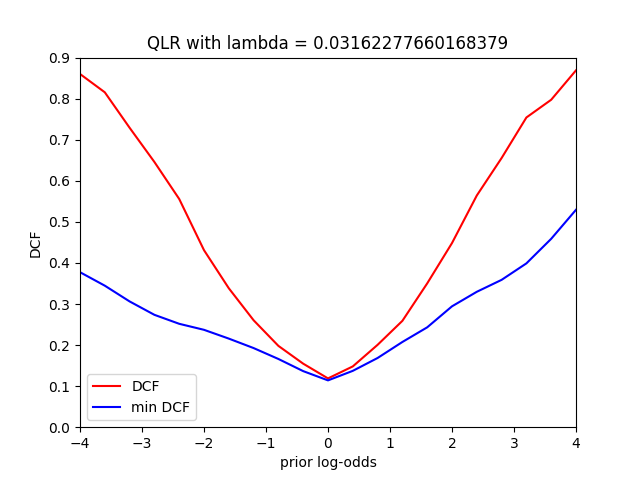
\includegraphics[width=\linewidth]{Lab/11. Lab 11/Images/BestConfiguration/01. QLR}
        \label{fig:QLRBest}
    \end{subfigure}
    \begin{subfigure}[b]{0.30\linewidth}
        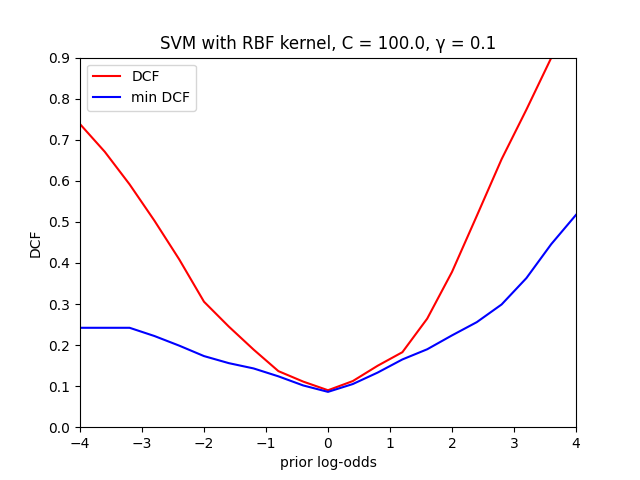
\includegraphics[width=\linewidth]{Lab/11. Lab 11/Images/BestConfiguration/02. SVM}
        \label{fig:SVM}
    \end{subfigure}
    \begin{subfigure}[b]{0.30\linewidth}
        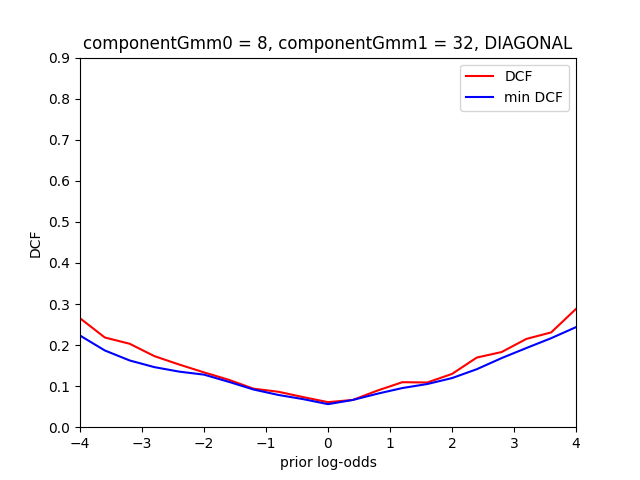
\includegraphics[width=\linewidth]{Lab/11. Lab 11/Images/BestConfiguration/03. GMM}
        \label{fig:GMM}
    \end{subfigure}
    \caption{Shows minDCF and actDCF for three best models}
    \label{fig:BestConfiguration}
\end{figure}

\subsection{Calibration Scores For Best Models}
\label{subsec:calibrationScores}

\begin{figure}[h!]
    \centering
    \begin{subfigure}[b]{0.40\linewidth}
        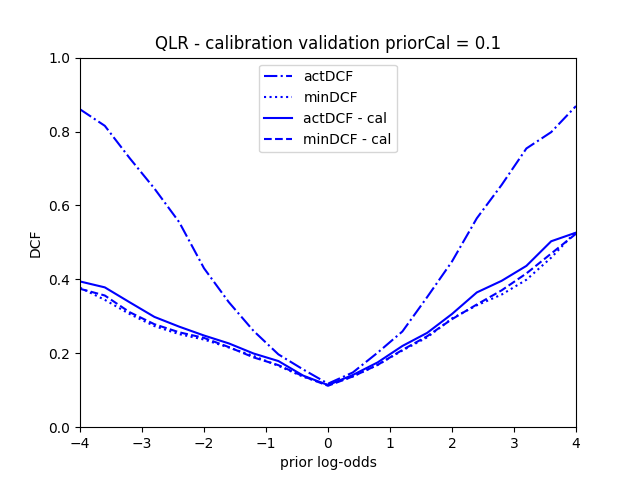
\includegraphics[width=\linewidth]{Lab/11. Lab 11/Images/CalibrationAndFusion/01. QLR}
        \label{fig:QLRCalibration}
    \end{subfigure}
    \begin{subfigure}[b]{0.40\linewidth}
        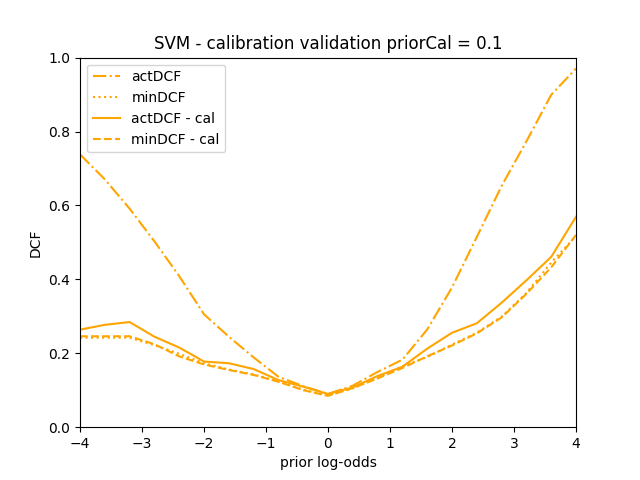
\includegraphics[width=\linewidth]{Lab/11. Lab 11/Images/CalibrationAndFusion/02. SVM}
        \label{fig:SVMCalibration}
    \end{subfigure}
    \begin{subfigure}[b]{0.40\linewidth}
        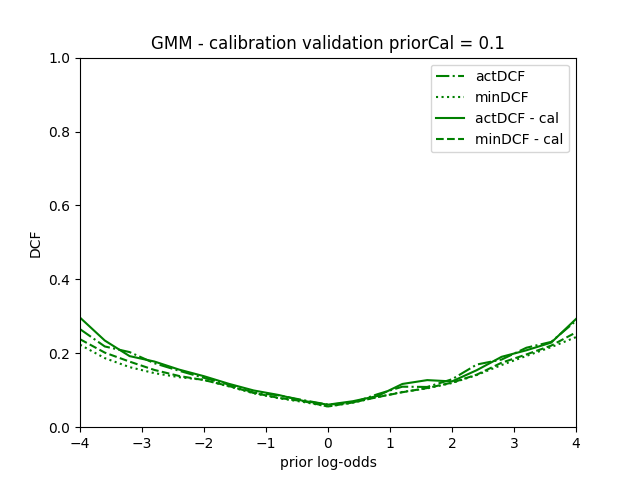
\includegraphics[width=\linewidth]{Lab/11. Lab 11/Images/CalibrationAndFusion/03. GMM}
        \label{fig:GMMCalibration}
    \end{subfigure}
    \begin{subfigure}[b]{0.40\linewidth}
        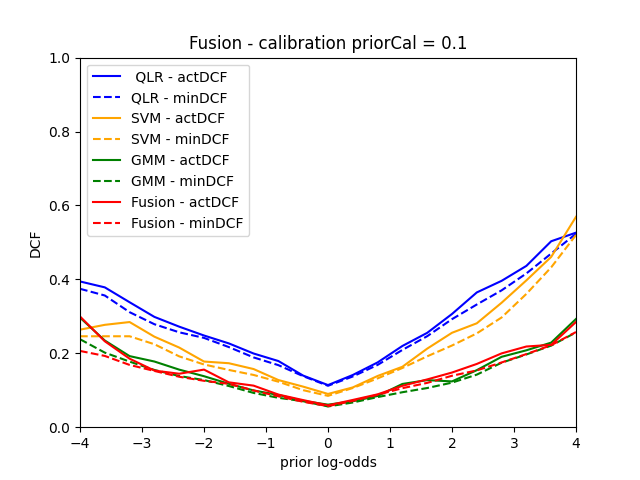
\includegraphics[width=\linewidth]{Lab/11. Lab 11/Images/CalibrationAndFusion/04. Fusion}
        \label{fig:FusionCalibration}
    \end{subfigure}
    \caption{Shows result of each model before and after calibration}
    \label{fig:BestConfigurationCalibration}
\end{figure}


\begin{table}[h!]
    \centering
    \begin{tabular}{>{\centering\arraybackslash}p{2.9cm} >{\centering\arraybackslash}p{2.9cm} >{\centering\arraybackslash}p{2.9cm} >{\centering\arraybackslash}p{2.9cm}}
        \toprule
        & \multicolumn{3}{c}{\textbf{Uncalibrated Models [minDCF - actDCF]}} \\
        \midrule
        \textbf{QLR} & \multicolumn{3}{c}{0.2436 - 0.4972} \\
        \textbf{SVM} & \multicolumn{3}{c}{0.1845 - 0.3581} \\
        \textbf{GMM} & \multicolumn{3}{c}{0.1312 - 0.1517} \\
        \midrule
        \midrule
        & \multicolumn{3}{c}{\textbf{Calibrated Models [minDCF - actDCF]}} \\
        \midrule
        & \(\tilde{\pi} = 0.1\) & \(\tilde{\pi} = 0.5\) & \(\tilde{\pi} = 0.9\) \\
        \midrule
        \textbf{QLR}    & 0.2486 - 0.2721       & 0.2496 - 0.2609       & 0.2480 - 0.2657       \\
        \textbf{SVM}    & 0.1794 - 0.1894       & 0.1814 - 0.2032       & 0.1881 - 0.2020       \\
        \textbf{GMM}    & 0.1324 - 0.1518       & 0.1314 - 0.1518       & 0.1283 - 0.1559       \\
        \midrule
        \textbf{Fusion} & 0.1304 - 0.1568       & 0.1373 - 0.1639       & 0.1382 - 0.1731       \\
        \bottomrule
    \end{tabular}
    \captionsetup{justification=justified,singlelinecheck=false,format=hang}
    \caption{Show minDCF and actDCF for different models before and after calibration}
    \label{tab:resultUnCalibratedAndCalibratedModels}
\end{table}
%
%
%\begin{table}[h!]
%    \centering
%    \begin{tabular}{>{\centering\arraybackslash}p{2.9cm} >{\centering\arraybackslash}p{2.9cm} >{\centering\arraybackslash}p{2.9cm} >{\centering\arraybackslash}p{2.9cm}}
%        \toprule
%        & \multicolumn{3}{c}{\textbf{Uncalibrated Models [minDCF - actDCF]}} \\
%        \midrule
%        \textbf{QLR} & \multicolumn{3}{c}{} \\
%        \textbf{SVM} & \multicolumn{3}{c}{} \\
%        \textbf{GMM} & \multicolumn{3}{c}{} \\
%        \midrule
%        \midrule
%        & \multicolumn{3}{c}{\textbf{Calibrated Models [minDCF - actDCF]}} \\
%        \midrule
%        & \(\tilde{\pi} = 0.1\) & \(\tilde{\pi} = 0.5\) & \(\tilde{\pi} = 0.9\) \\
%        \midrule
%        \textbf{QLR}    &                       &                       &                       \\
%        \textbf{SVM}    &                       &                       &                       \\
%        \textbf{GMM}    &                       &                       &                       \\
%        \midrule
%        \textbf{Fusion} &                       &                       &                       \\
%        \bottomrule
%    \end{tabular}
%    \captionsetup{justification=justified,singlelinecheck=false,format=hang}
%    \caption{Show minDCF and actDCF for different models before and after calibration on eval dataset}
%    \label{tab:resultUnCalibratedAndCalibratedModelsOnEval}
%\end{table}


    \section{Experimental Results}
    \label{sec:experimentalResults}
    %! Author = antonio
%! Date = 9/6/24

\subsection{Evaluation}
\label{subsec:evaluation}

Starting with the model already tested, we go on to see how it behaves with another dataset which is the evaluation dataset.

\begin{figure}[h!]
    \centering
    \begin{subfigure}[b]{0.40\linewidth}
        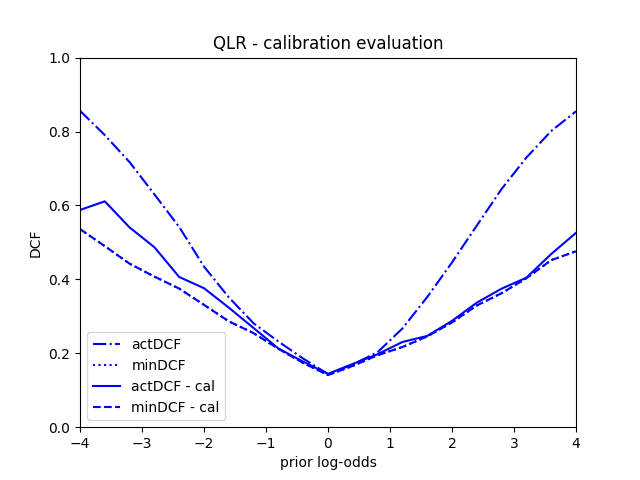
\includegraphics[width=\linewidth]{Lab/11. Lab 11/Images/Evaluation/01. QLR}
        \label{fig:QLREvaluation}
    \end{subfigure}
    \begin{subfigure}[b]{0.40\linewidth}
        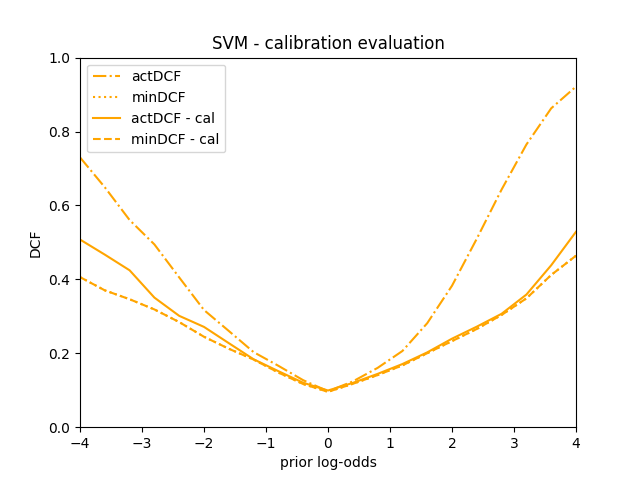
\includegraphics[width=\linewidth]{Lab/11. Lab 11/Images/Evaluation/02. SVM}
        \label{fig:SVMEvaluation}
    \end{subfigure}
    \begin{subfigure}[b]{0.40\linewidth}
        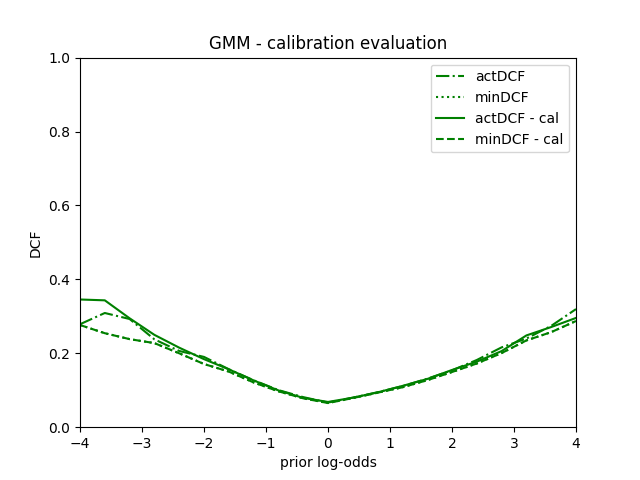
\includegraphics[width=\linewidth]{Lab/11. Lab 11/Images/Evaluation/03. GMM}
        \label{fig:GMMEvaluation}
    \end{subfigure}
    \begin{subfigure}[b]{0.40\linewidth}
        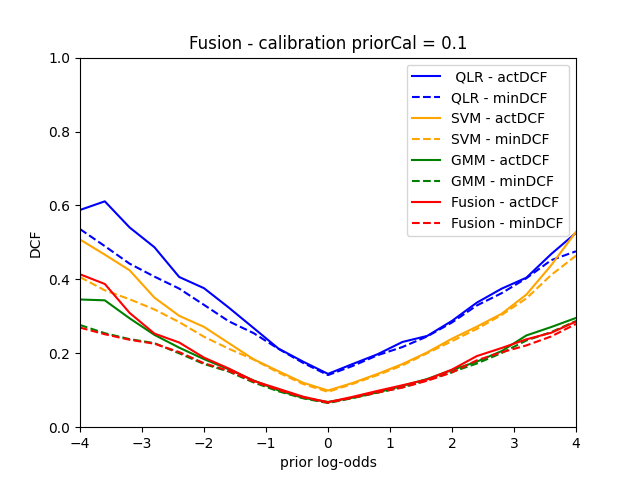
\includegraphics[width=\linewidth]{Lab/11. Lab 11/Images/Evaluation/04. Fusion}
        \label{fig:FusionEvaluation}
    \end{subfigure}
    \caption{Shows result of each model before and after calibration with the evaluation dataset}
    \label{fig:BestConfigurationCalibrationEvaluation}
\end{figure}

The \autoref{fig:BestConfigurationCalibrationEvaluation} shows the result of each model before and after calibration with the evaluation dataset
and a \(\tilde{\pi} = 0.1\).

\begin{table}[h!]
    \centering
    \begin{tabular}{>{\centering\arraybackslash}p{2.9cm} >{\centering\arraybackslash}p{2.9cm} >{\centering\arraybackslash}p{2.9cm} >{\centering\arraybackslash}p{2.9cm}}
        \toprule
        & \multicolumn{3}{c}{\textbf{Uncalibrated Models [minDCF - actDCF]}} \\
        \midrule
        \textbf{QLR} & \multicolumn{3}{c}{0.3515 - 0.4935} \\
        \textbf{SVM} & \multicolumn{3}{c}{0.2636 - 0.3634} \\
        \textbf{GMM} & \multicolumn{3}{c}{0.1838 - 0.1953} \\
        \midrule
        \midrule
        & \multicolumn{3}{c}{\textbf{Calibrated Models [minDCF - actDCF]}} \\
        \midrule
        & \(\tilde{\pi} = 0.1\) & \(\tilde{\pi} = 0.5\) & \(\tilde{\pi} = 0.9\) \\
        \midrule
        \textbf{QLR}    & 0.3515 - 0.3896       & 0.3515 - 0.3717       & 0.3515 - 0.3648       \\
        \textbf{SVM}    & 0.2636 - 0.2939       & 0.2636 - 0.2714       & 0.2636 - 0.2695       \\
        \textbf{GMM}    & 0.1838 - 0.2053       & 0.1838 - 0.2023       & 0.1838 - 0.2106       \\
        \midrule
        \textbf{Fusion} & 0.1865 - 0.2046       & 0.1831 - 0.2056       & 0.1828 - 0.2089       \\
        \bottomrule
    \end{tabular}
    \captionsetup{justification=justified,singlelinecheck=false,format=hang}
    \caption{Show minDCF and actDCF for different models before and after calibration on eval dataset}
    \label{tab:resultUnCalibratedAndCalibratedModelsOnEval}
\end{table}

The \autoref{tab:resultUnCalibratedAndCalibratedModelsOnEval} shows the minDCF and actDCF for different models before and
after calibration on the evaluation dataset.
From the values obtained, it is confirmed that GMM is again the method that gives the best performance, but Fusion also
gives good results that do not deviate much from those of GMM.


    \section{Conclusion}
    \label{sec:conclusion}
    %! Author = antonio
%! Date = 9/6/24

Concluding our experiment, it can be observed that quadratic models perform better.
Furthermore, among these models, it can be seen that those that make assumptions about the independence of the features don't lose performance,
which means that the features are indeed not particularly correlated, and this is also confirmed by the GMM model, the best performing,
that the features can be considered independent of each other.\\
Following on from what has been said about features independence, it can be seen that PCA did not lead to any real improvement,
these might be possible because the original features are already independent and contribute uniformly to the variance of the data,
hence PCA might not improve performance.
This is because PCA may be useful when there are relationships between features that could be exploited to reduce dimensionality,
but when this relationship does not exist, each component carries with it a small part of the total variance,
thus making the application of PCA of little use.
In conclusion, it can be said that the considerations made on our model, based on the training dataset, also proved useful on the evaluation dataset.
In fact, the model chosen was the one that performed best on the latter dataset as well.


\end{document}
